%\chapter{The "selector"}
\section{Problem statement}
Let's consider, as concrete examples, a 3d hill geometry of Fig.~\ref{fig:examples}a or a submarine model with full appendages of Fig.~\ref{fig:examples}b.

\begin{figure}[H]%
    \centering
    \subfloat[\centering The (BeVERLI) hill geometry.]{{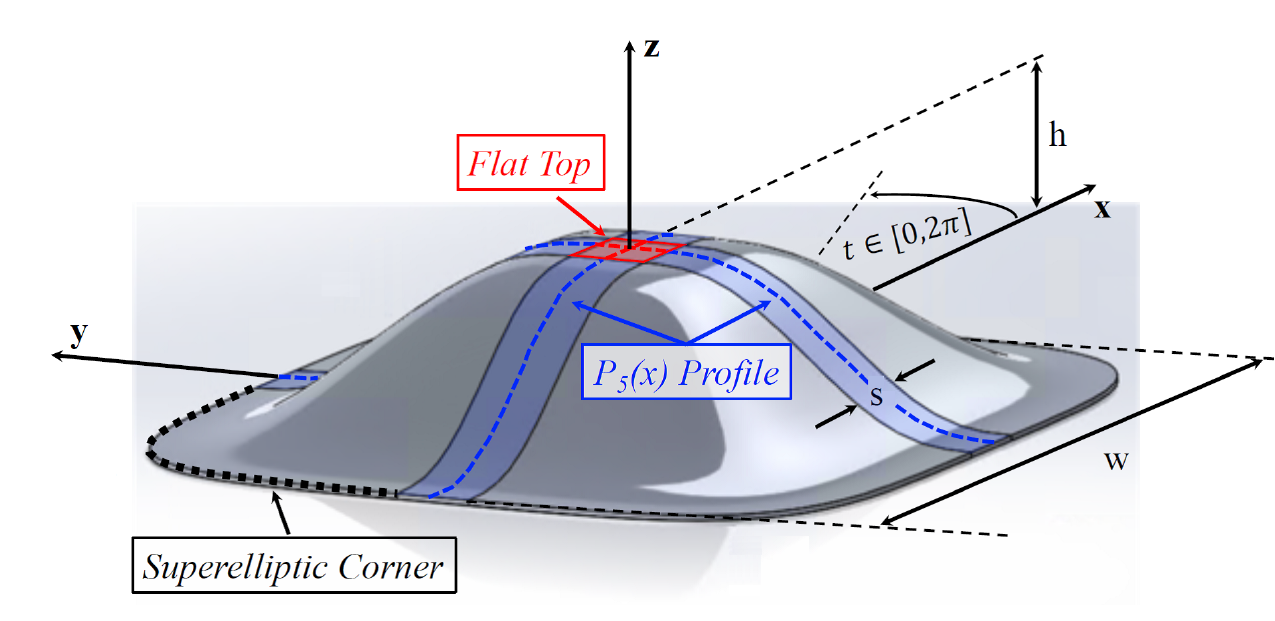
\includegraphics[width=0.45\textwidth]{figs/hill.png}}}%
    \qquad
    \subfloat[\centering A generic (BB2) submarine.]{{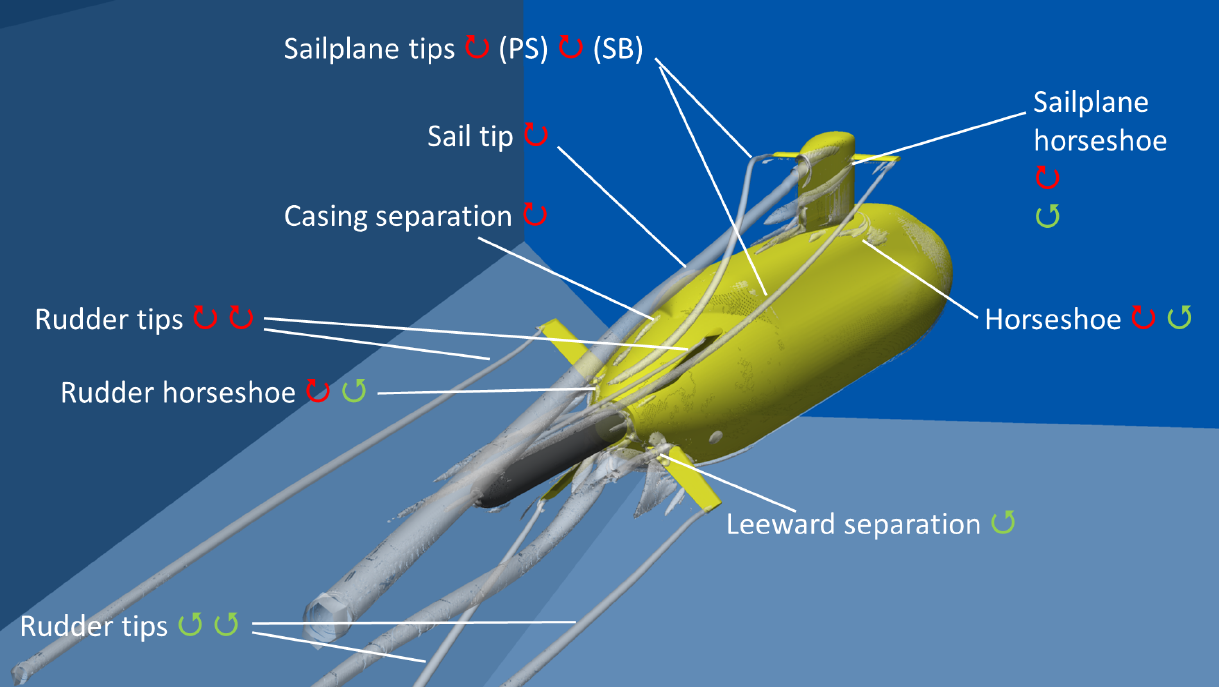
\includegraphics[width=0.45\textwidth]{figs/submarine.png}}}%
    \caption{Examples of non-canonical 3d flows.}%
    \label{fig:examples}%
\end{figure}

\noindent As known from the examples above, different regions of the flow field are characterized by different flow structures, patterns and topology. It is, thus, reasonable to expect that a dedicated model which better reproduces such physics in each region, may improve the global representativity of the simulation. Then, the general definition of the problem can be as follows:
\textcolor{red}{(T1) given a set of GEP models developed for different \textbf{canonical} flows, \textbf{automatically} select the \textbf{best} model in each region of the computational domain for a \textbf{new and unseen}, possibly non-canonical testcase.}

\vspace{10pt}
\noindent There are few keywords to notice in the definition above, which identify several sub-tasks:
\paragraph{Canonical flows.} (ST1) Currently, the available GEP\index{GEP} models have been developed for the following testcases:
\begin{itemize}
    \item 3d square cylinder
    \item 2d airfoil
    \item backfacing step
    \item impinging jet
    \item ...
    \item \textcolor{blue}{experimental or high-fidelity data?}
\end{itemize}
Baseline and GEP\index{GEP}-improved solutions should be available for each testcase. Is it also worth noticing here the importance of the \textbf{identification and selection features and targets} (QoI) for each testcase. These will make up the database which the machine learning algorithm will work on. 

\paragraph{Automatically.} (ST2) We would like to minimize or nullify the human intervention in the model's selection and assignment process. This points to the adoption of a machine or deep learning framework. \textcolor{blue}{Nevertheless, it may be that more traditional methods such as shock/vortex features filters/detectors would be enough?}

\paragraph{Best model.} (ST3) The notion of "best" implies the definition of some metric able to estimate the quality/similarity/correlation between the models available and the flow currently under assessment.

\paragraph{New and unseen.} (ST4) This points to the choice between supervised and unsupervised approach. Given a comparable accuracy between the two methodologies, preference shall be given to unsupervised algorithms in order to get rid of the heavy training phase, as well as the compilation of a database. 

\vspace{10pt}
\noindent Once the aforementioned sub-tasks are fulfilled, the next key question (also from navy guys) is: \textcolor{red}{(T2) how to "blend" different models from different regions?} and consequently how to call and apply each model from the main solver.

\section{The "selector" concept}
In this section, some ideas about how to realize such "model selector" are presented.

\subsection{Data structure}
\textit{The actual implementation of the "selector" appears to be dependent on the type of data structure we are going to process.} Specifically, given the numerical solution of the testcase shall we consider:
\begin{itemize}
    \item 1D data sets (extracted from \index{OpenFOAM@\hypertarget{OpenFOAM.ind}{}OpenFOAM}\href{\#OpenFOAM.ind}{OpenFOAM})
    \item 2D surfaces data (extracted from \index{OpenFOAM@\hypertarget{OpenFOAM.ind}{}OpenFOAM}\href{\#OpenFOAM.ind}{OpenFOAM})
    \item fully 3D data (exported raw solution)
\end{itemize}
Typically, machine and deep learning algorithms are specialized to deal with one preferred data format, thus, \textit{different workflows should be defined depending on the data structure}. 

\textit{Thinking about an "in the loop" approach, it is worth noticing that sets and surfaces are much more "manageable" but are (only?) available at post-processing time while fully 3D data may be available at each solution save time but it requires considerable more time to be processed, if used in toto.}

\subsection{Machine/deep learning algorithm}
Another choice to be made is the selection of the class of algorithms to be employed for the task, namely, supervised or unsupervised (self-supervised, weakly-supervised). 
As stated above, the priority would be given to unsupervised machine learning algorithms in order to avoid the need of large-scale labelled datasets and eventually the associated training process. Consequently, the attention will be "naturally" focused on techniques such as \underline{\textbf{unsupervised} \textbf{clustering}\index{clustering} and \textbf{segmentation}\index{segmentation}}. 
 
\textbf{Cluster\index{clustering} analysis} or clustering\index{clustering} is the task of grouping a set of objects in such a way that objects in the same group (called a cluster\index{clustering}) are more similar (in some sense) to each other than to those in other groups (clusters\index{clustering})\footnote{https://en.wikipedia.org/wiki/Cluster\_analysis}. The objective of clustering is to organise data so that the inner-cluster similarity is maximised while the inter-cluster\index{clustering} similarity is minimised~\cite{kaiser2014cluster}. 
 
\textbf{Semantic segmentation} is the process of classifying each individual pixel of an image into a known ontology~\cite{hamilton2022unsupervised} or equivalently, assigning a class label to every pixel of an image~\cite{van2021unsupervised}. Moreover, if semantic segmentation predicts the labels for every pixel in the input image and each pixel is labelled according to the object class within which it is enclosed, \textbf{instance segmentation} gives different labels for separate instances of objects belonging to the same class. Hence, instance segmentation simultaneously solves the problem of object detection as well as that of semantic segmentation~\cite{hafiz2020survey}. Reasonably, cluster analysis, semantic and instance segmentation shared some common features and they are often used together.

\vspace{10pt}
\noindent \textcolor{blue}{It is worth observing that, the pixel-level classification and segmentation, perhaps, solves the second task (T2) concerning the blending strategy of different models between different regions of the domain. Indeed, having a pixel-by-pixel description would allow to seamlessly assign the model according to the class or segment the pixel belongs to (expensive strategy). More efficiently, an additional field variable may be instantiated in OF, for example, a integer vector with length equal to the number of sub-volumes or models, as well. This will be initialized at t=0, but eventually, it could be read at run time. In this way, it could be re-assigned to a different model.}

\subsubsection{Segmentation of turbulent computational fluid dynamics simulations with
unsupervised ensemble learning~\cite{bussov2021segmentation}}
In~\cite{bussov2021segmentation} an unsupervised clustering ensemble learning technique is used to perform the segmentation of turbulent flow field. From Fig.~\ref{fig:papersconnected}, it is interesting to observe that apparently no other prior or derivative works have dealt with segmentation and clustering of fluid dynamic flow fields and such work appears quite isolated. 

\vspace{10pt}
\noindent According to~\cite{bussov2021segmentation} a workflow with the following features\footnote{\url{https://github.com/mkruuse/segmenting-turbulent-simulations-with-ensemble-learning}} can be devised:
\begin{itemize}
    \item computer vision and machine learning tools are adopted to automate the segmentation of physical structures from 2-dimensional image snapshots 
    \item machine learning clustering algorithms are used for detection and segmentation of visually distinct structures in data (fast enough to be coupled directly into time simulation loop
    \item SCE algorithm is used to average segmentation results from many independent clustering realizations (obtained via SOM algorithm) in order to mitigate the non-deterministic nature of clustering algorithms (influence of initial conditions and different parameters) and obtaining more accurate ROI objects
    \item determine optimal number of meaningful clusters present in the input data
    \item uniquely identify each pixel with the corresponding object cluster
    \item segment clustered pixels into stable contours that can be further analyzed for their geometrical shape, size, and area
    \item each individual clustering realization can be split into different image masks where only the pixels from one specific cluster are "active". Stacking operations of these masks are defined by using the union, intersection, and sum of two masks.
\end{itemize}
%
\begin{figure}[H]%
    \centering
    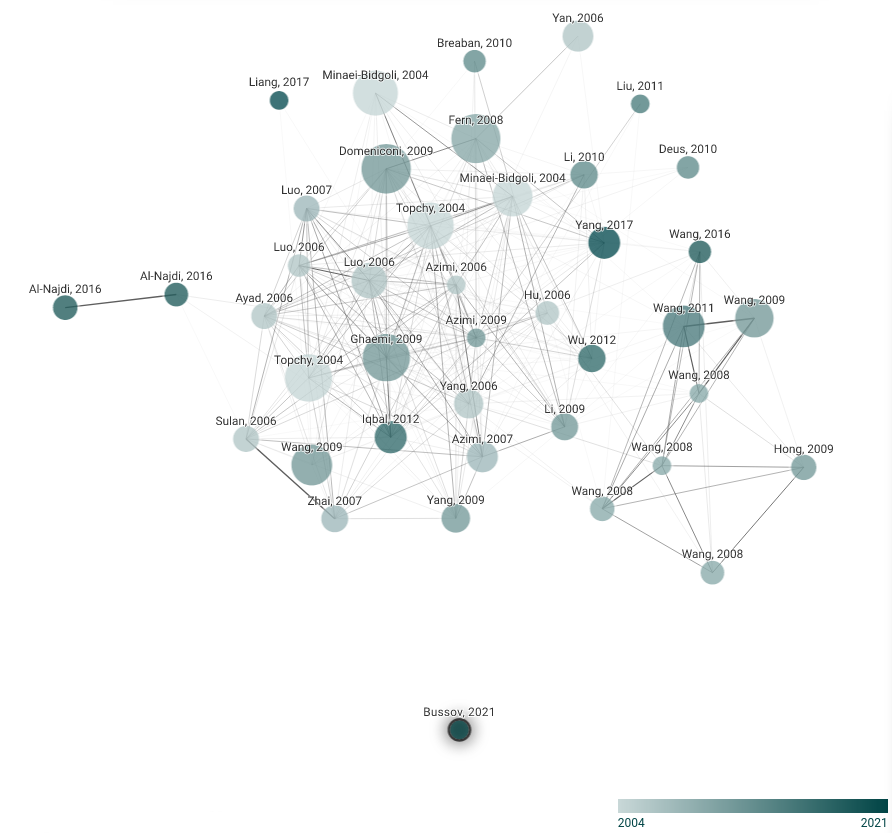
\includegraphics[width=0.7\textwidth]{figs/papersconnected.png}
    \caption{Visual graph of connected papers for~\cite{bussov2021segmentation}.}
    \label{fig:papersconnected}%
\end{figure}
%
Some other works~\cite{van2021unsupervised,hamilton2022unsupervised,ji2019invariant,caron2018deep} proposed even more effective and efficient segmentation and clustering\index{clustering} techniques, nevertheless not targeted for fluid dynamic applications. In~\cite{kaiser2014cluster}, a cluster-based reduced-order modelling of a mixing layer was considered. An increasing number of publications adopting segmentation and clustering techniques for medical imagine application, can be found in literature, such as~\cite{colebank2019influence}.

\subsubsection{Deep learning for 3D point clouds: a survey~\cite{guo2020deep}}
If we accept to abandon or at least partially deviate from the choice of using strictly only unsupervised algorithms, we number of publications increases significantly. In particular, if we retain the idea of working with 3D data (no extracted sets or surfaces from OF) we need consider algorithms able to handle clouds of points~\ref{fig:taxo}. In this regards, very informative is the recent review~\cite{guo2020deep} whose visual graph of connected papers is reported in Fig.~\ref{fig:guo}. The impact of such publication is apparent from the size of the corresponding circle as well as the rich network of citations.
%
\begin{figure}[H]%
    \centering
    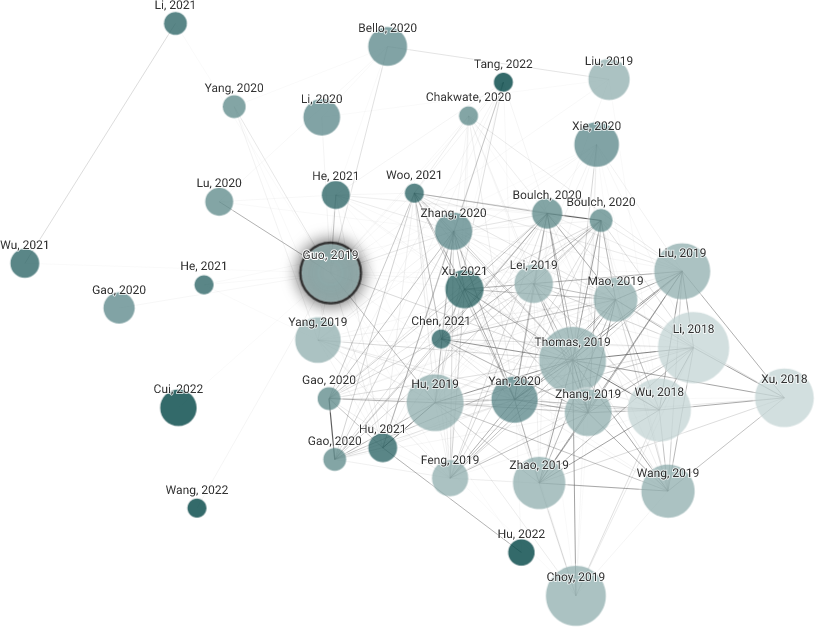
\includegraphics[width=0.7\textwidth]{figs/guo.png}
    \caption{Visual graph of connected papers for~\cite{guo2020deep}.}
    \label{fig:guo}%
\end{figure}
%
\noindent From~\cite{guo2020deep}, many different methods and architectures can be adopted for our task, in terms of classification, clustering, detection and segmentation. In particular, as suggested in~\cite{sun2021automated}, the following automated simulation framework data-driven turbulence modeling workflow can be developed:
\begin{enumerate}
    \item Data acquisition and preprocessing (OF solutions).
    \item Point cloud segmentation based on deep learning: perform a semantic segmentation of the point clouds, which divides the point clouds according to their physical significance. A filter may be applied at this stage (Gabor, Sobel, ...). Subsequently, the point clouds are segmented using deep learning, (possibly reducing the work of feature engineering and enhancing the capture of local features). The method may combine 2D network, (DeepLabv3)\footnote{https://paperswithcode.com/method/deeplabv3}, and 3D network, (PointNet++)\footnote{https://paperswithcode.com/paper/pointnet-deep-hierarchical-feature-learning}. The point clouds are first rasterized into 2D images as the input of DeepLabv3, which subsequently predicts the probability vectors of pixel-by-pixel classification and maps them back to the points. Finally, the point clouds are sparsified and input into PointNet++ to obtain point-by-point classification results.
    \item Geometric 3D reconstruction: after obtaining the respective point clouds, it is necessary to establish clean and low-complexity models of the target area, which are suitable for CFD simulation.
    \item CFD modeling and simulation: the 3D models in STL format generated for each sub-region are directly imported into OF. Grids are generated using its automatic grid generation function. To perform a CFD simulation, the sub-regions are assigned different GEP model (if necessary w.r.t. the baseline) by implementing an automated script based on the labels identified by the clustering phase.
\end{enumerate}

\begin{sidewaysfigure}
    \centering
    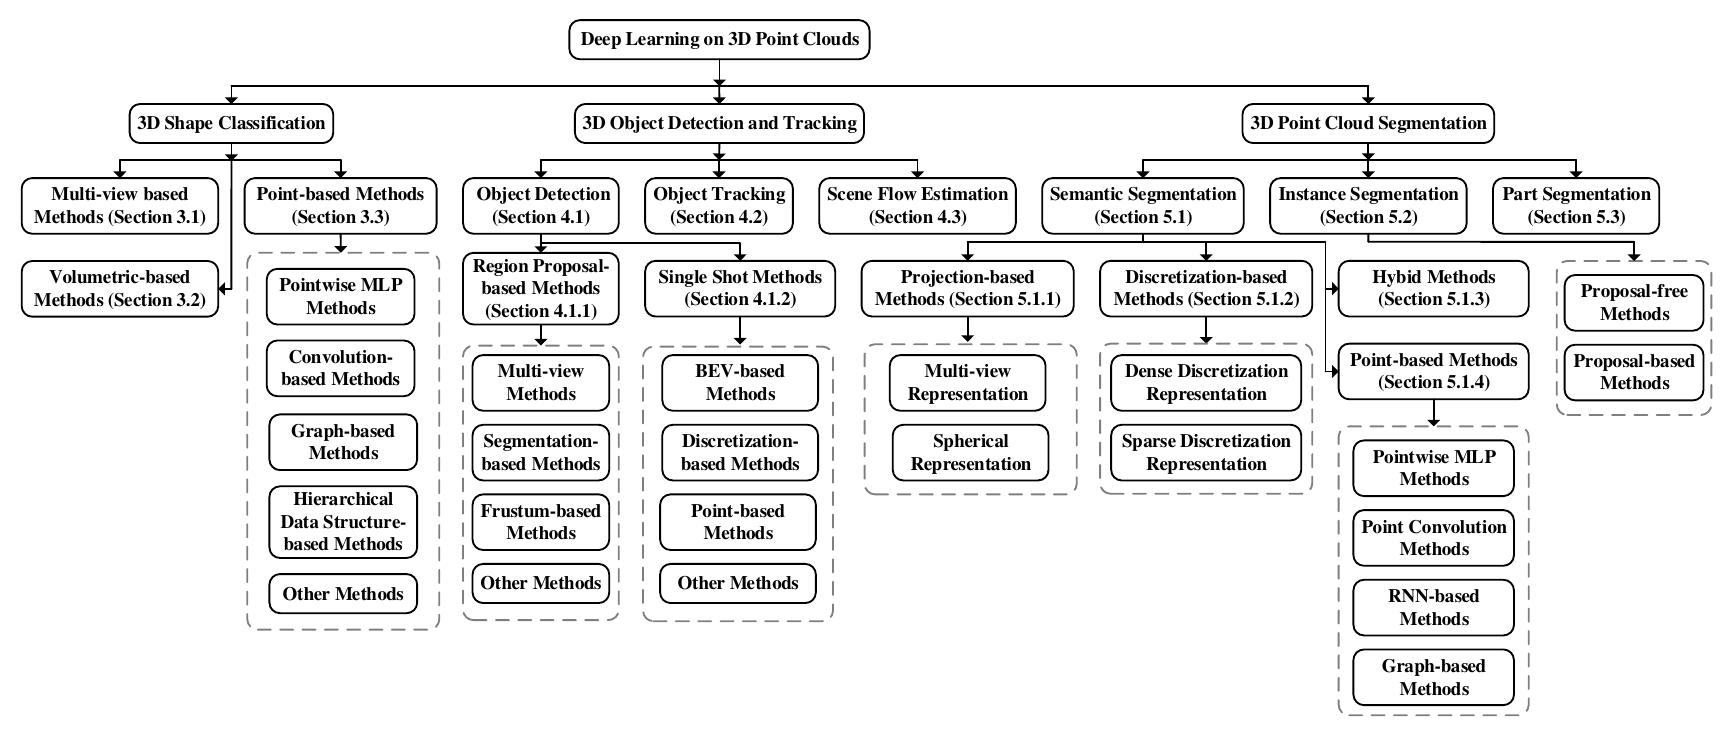
\includegraphics[width=1.0\textwidth]{figs/taxonomy.png}
    \caption{A taxonomy of deep learning methods for 3D point clouds~\cite{guo2020deep}.}
    \label{fig:taxo}%
\end{sidewaysfigure}

\subsubsection{Unsupervised Semantic Segmentation by Distilling Feature Correspondences}
\url{https://github.com/mhamilton723/STEGO}\\
\url{https://github.com/facebookresearch/dino}\\
\url{https://github.com/facebookresearch/DeeperCluster}\\
\url{https://github.com/facebookresearch/swav}\\

\begin{figure}
    \centering
    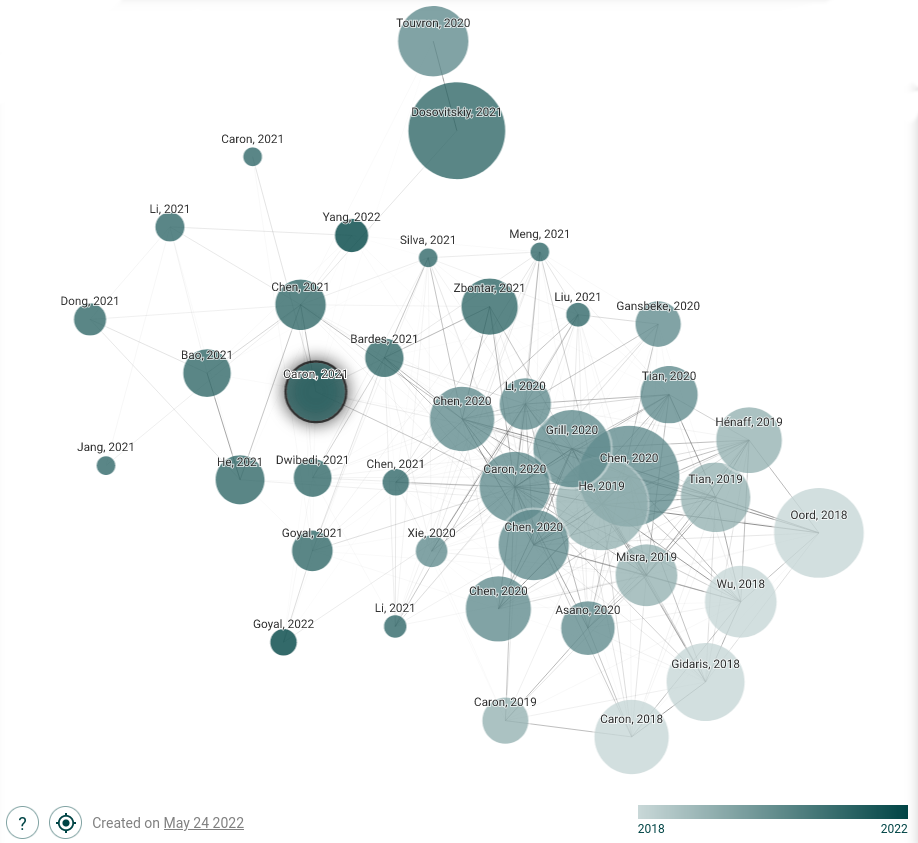
\includegraphics[width=0.75\textwidth]{figs/dino.png}
    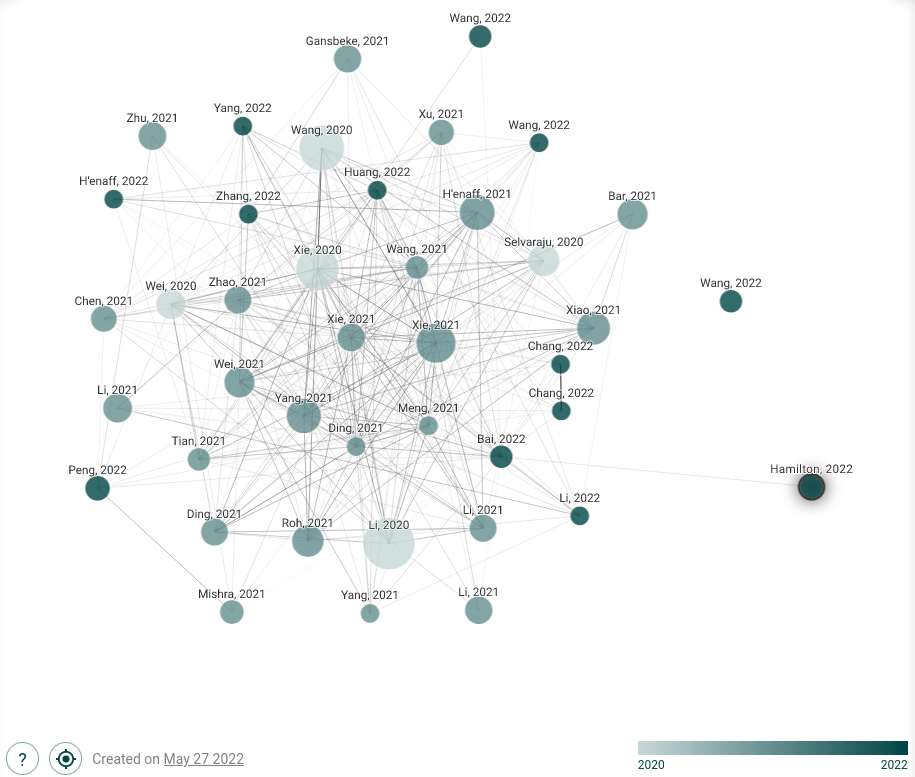
\includegraphics[width=0.75\textwidth]{figs/stego.png}
    \caption{Visual graph of connected papers for DINO~\cite{caron2021emerging} and STEGO~\cite{hamilton2022unsupervised}.}
    \label{fig:DINO_STEGO}%
\end{figure}

\subsection{Clustering}
%https://www.r-bloggers.com/2019/01/10-tips-for-choosing-the-optimal-number-of-clusters/
In this section, the progress about clustering analysis for data-driven turbulence modeling will be reported. A general overview on this class of algorithms can be found in~\cite{bouveyron2019model,giordani2020introduction,skiadas2019data}.

It should be soon realised that the clustering\index{clustering} problem which we are tackling is far more challenging than traditional examples. Indeed, if for example consider the typical Iris database~\ref{tab:iris}, we have only four features and three species to be clustered, while in our case we may possibly have more targets corresponding to each point of the computational domain to be clustered and each point has many more features which it may depend upon, corresponding to the QoI from the flow field solution, as exemplified in~\ref{tab:reality}. Thus, at least in the present formulation, the problem will certainly benefit from a \textbf{dimensionality reduction} as well as a \textbf{feature selection} pre-processing step.
%
\begin{table}[H]
\begin{centering}
\begin{tabular}{ccccc}
Sepal.length & Sepal.width & Petal.length & Petal.width & Species\tabularnewline
\hline
\hline
. & . & . & . & setosa\tabularnewline
\hline
. & . & . & . & virginica\tabularnewline
\hline
. & . & . & . & versicolor\tabularnewline
\hline
\end{tabular}
\par\end{centering}
\caption{\label{tab:iris}Exemplification of Iris database}
\end{table}
%
\begin{table}[H]
\begin{centering}
\begin{tabular}{cccccccccc}
$a_{ij}\left[6\right]$ & $R\left[6\right]$ & \textbf{$u\left[3\right]$} & $I_{i}\left[5\right]$ & $T_{i}\left[10\right]$ & k & $\omega$ & $\nu_{t}$ & ... & Points\tabularnewline
\hline
\hline
. & . & . & . & . & . & . & . & . & 1\tabularnewline
\hline
. & . & . & . & . & . & . & . & . & 2\tabularnewline
\hline
. & . & . & . & . & . & . & . & . & .\tabularnewline
\hline
. & . & . & . & . & . & . & . & . & n\tabularnewline
\hline
\end{tabular}
\par\end{centering}
\caption{\label{tab:reality}Example of a realistic database}
\end{table}

%\vspace{10pt}
%Some interesting projects are reported below:\\
%\url{https://github.com/xu-ji/IIC} \\
%\url{https://github.com/wvangansbeke/Unsupervised-Semantic-Segmentation} \\
%\url{https://github.com/mhamilton723/STEGO} \\
%\url{https://github.com/hbilen/wsl-eccv20.github.io} \\
%\url{https://github.com/facebookresearch/moco/fork} \\
%\url{https://github.com/facebookresearch/swav} \\
%\url{https://github.com/facebookresearch/deepcluster}

\subsection{Unsupervised detection, segmentation and clustering}
As preferred choice, an unsupervised approach will be pursued. In particular, a three-dimensional unsupervised clustering method will be sought. In this regards, the review paper~\cite{xiao2022unsupervised} is of particular interest\footnote{\url{https://github.com/xiaoaoran/3d_url_survey}}.

\subsection{Dimensionality reduction}
One immediate issue which arises from the high-dimensionality of the database is to visualize or more precisely to find an appropriate mapping to a two- or three-dimensional space which preserves pairwise similarities as well as possible. 

Among the wide range of choice\footnote{https://scikit-learn.org/stable/modules/decomposition.html\#decompositions},\footnote{https://scikit-learn.org/stable/modules/manifold.html}, an interesting option seems to be the t-SNE algorithm~\cite{van2008visualizing} due to its properties. The main idea behind t-SNE\index{t-SNE} is to map a high-dimensional space $X$ to a low-dimensional space $Y$ where the distribution of pairwise similarities is preserved as much as possible. Similarity between data points $x_i$, $x_j$ $\in$ $X$ is defined as the probability that $x_i$ would pick $x_j$ as its neighbor. A similar probability distribution is found in $Y$ by minimizing the Kullback-Leibler divergence between the two distributions
using gradient descent. 

% https://stats.stackexchange.com/questions/263539/clustering-on-the-output-of-t-sne
Nevertheless, t-SNE\index{t-SNE} does not preserve distances nor density. It only to some extent preserves nearest-neighbors. The difference is subtle, but affects any density- or distance-based algorithms.
While clustering after t-SNE\index{t-SNE} will sometimes (often?) work, it may be difficult to explain the clusters, as we may just see 'shapes in clouds' not necessarily clear whether real or artifacts. Therefore, applying any clustering algorithms after t-SNE\index{t-SNE} may not be a good starting point since the initial data may be heavily distorted, and neither distances nor density are preserved well.

At present, a viable option seems to be LargeVis~\cite{tang2016visualizing} which implements an optimized version of t-SNE\index{t-SNE} and reports good scalability properties.

\section{Workflow}
At the moment the preferred framework to compare clustering algorithms is R~\cite{team2013r} as well as the implementation of scikit-learn~\cite{pedregosa2011scikit}. The two environments are compatible with each other and conversion into one or another is easily done.

\vspace{10pt}
\noindent The adopted workflow is the following:
\begin{itemize}
    \item Consider the solution or the surface data extracted at the last time. Extracted surfaces are somehow better because they include the position coordinates. Moreover, the exporting of the solution as a spreadsheet can be quite long for refined meshes and a large number of variables.
    \item Convert it to a \texttt{csv} file which will constitute the database for the further clustering. This step is performed by running a script which saves all the QoI from different planes of the computational domain in corresponding files.
    \item An itermediate pre-processing step may be included in order to concatenate/split different solution fields (input features) into one/several files. At this stage, feature selection or model reduction may be applied.
    \item Run clustering algorithm for each testcase (canonical and current). {As result from the clustering and/or segmentation analysis, we will have a certain number of clusters containing a three-dimensional portion of the domain whose points are labelled according to their physical meaning.} 
    \item Once the list of points for each region and their physical labels are known for the target simulation, they can be compared with the canonicals' ones to compute a "similarity metrics". The best performing metric will identify which model should be used for each sub-region.
    \item The list of points for each sub-region, their physical labels and the metric can be imported into the solver and used to select and assign the model.
\end{itemize}

\vspace{10pt}
\underline{Among unknown ones, few possible issues and observations ...}
\begin{itemize}
\item Three-dimensional nature of the domain, while clustering analysis is typically applied on two-dimensional planes.
\item Complex flow topology, as shown in Fig.~\ref{fig:streamlines}, which makes difficult to obtain a clean clustering or closed surfaces to be directly imported in OF (some filtering may be necessary).
\item Size of the simulations make post-processing and/or conversions quite resources consuming (this would point to minimal end-to-end interference).
\item Baseline or the GEP-augmented solution should be used? In any case, a fixed set of variables should be selected for the machine learning "filtering" stage (this points to a feature importance analysis for each testcase).
\item \textcolor{green}{The final output of the clustering/segmentation processing stage could be an STL surface which encapsulates a sub-volume region of the full domain. The number of these sub-volumes should correspond to the number of available models to be selected. Thus, an additional field variable may be instantiated in OF, for example, a integer vector with length equal to the number of sub-volumes or models, as well. This will be initialized at t=0, but eventually, it could be read at run time. In this way, it could be re-assigned to a different model.}
\end{itemize}

\begin{figure}[H]%
    \centering
    \subfloat[\centering velocity gradient magnitude]{{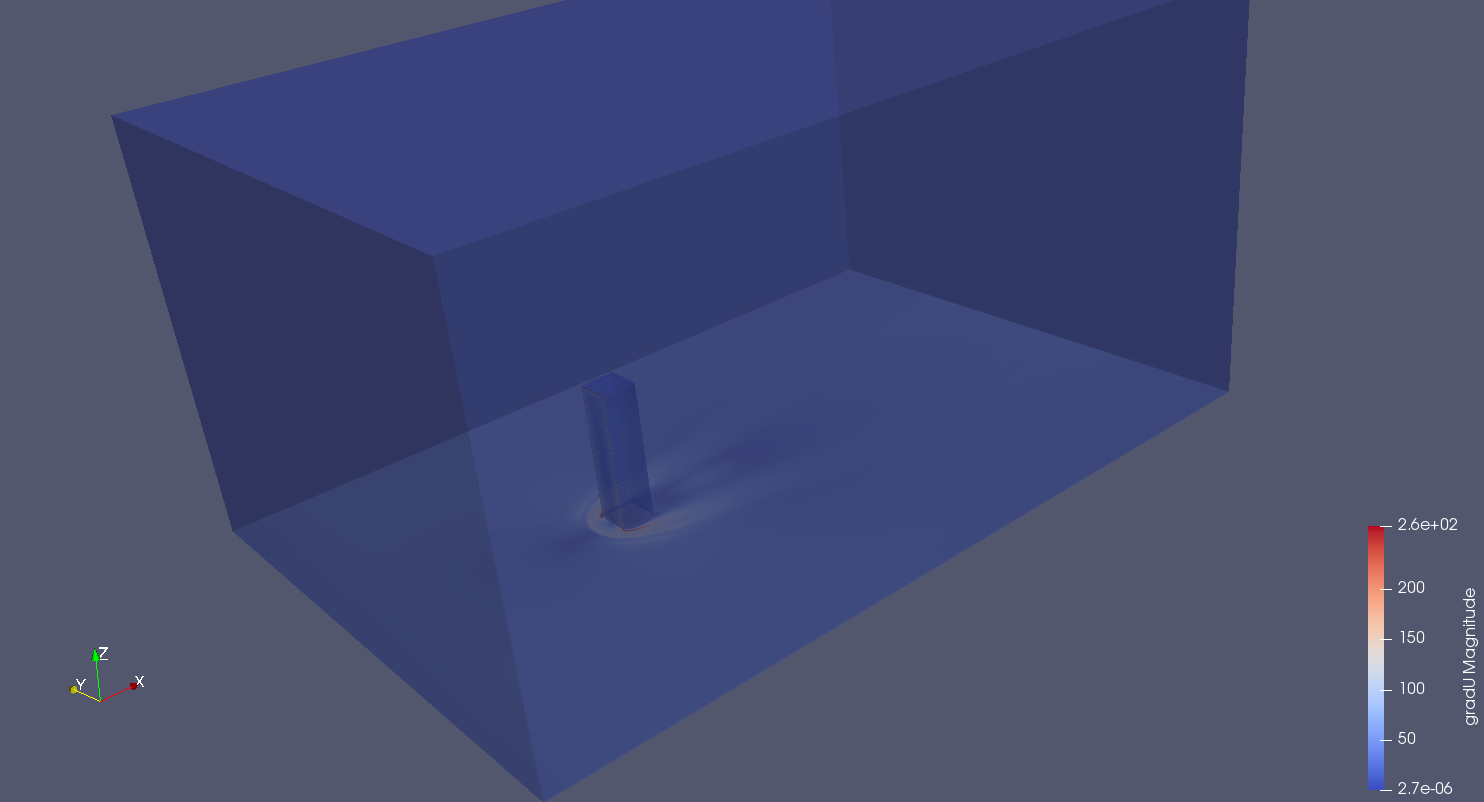
\includegraphics[width=0.45\textwidth]{figs/sqcyl/gradU.png}}}%
    \qquad
    \subfloat[\centering velocity magnitude]{{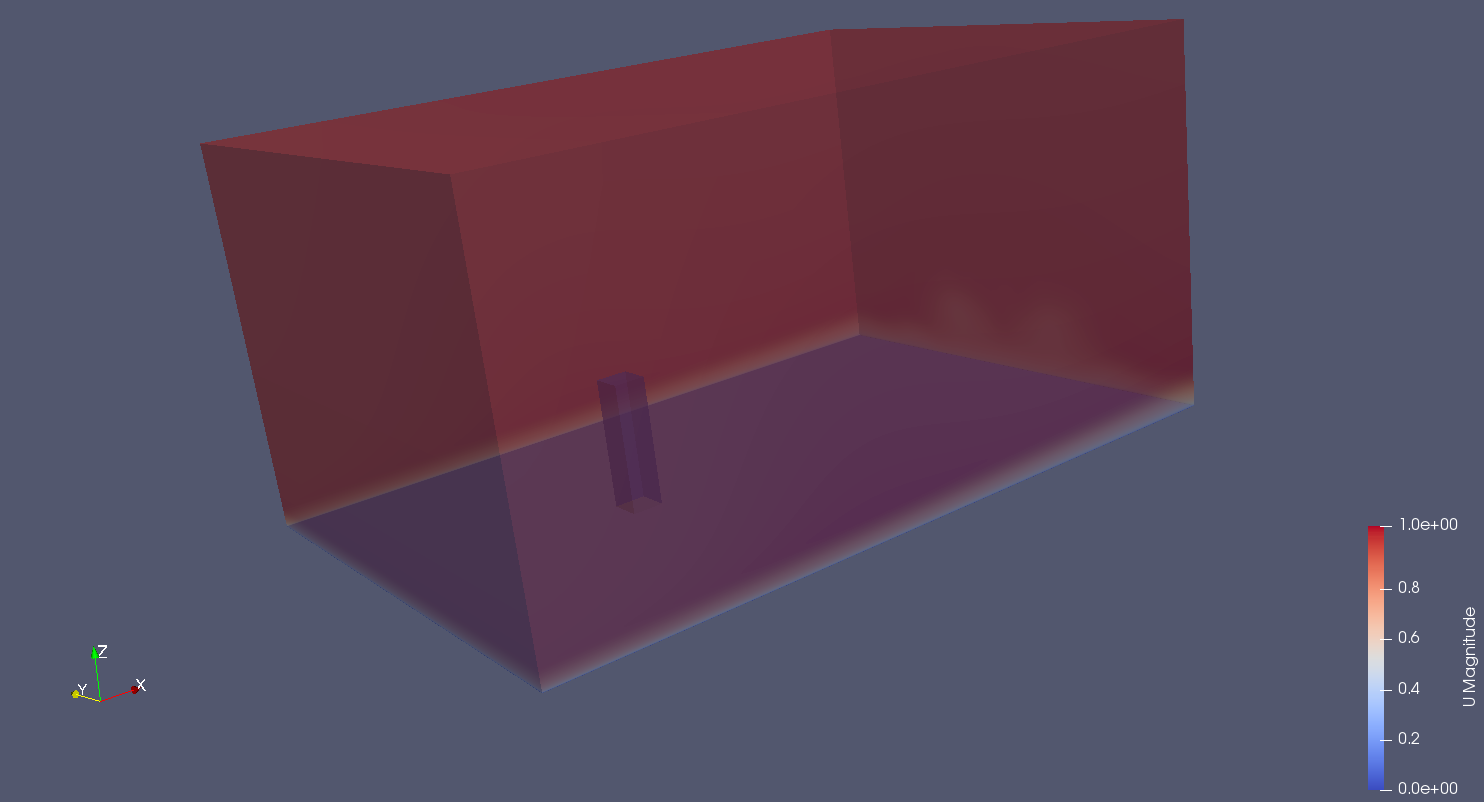
\includegraphics[width=0.45\textwidth]{figs/sqcyl/U.png}}}%
    \caption{}%
    \subfloat[\centering $a_{ij}^x$ magnitude]{{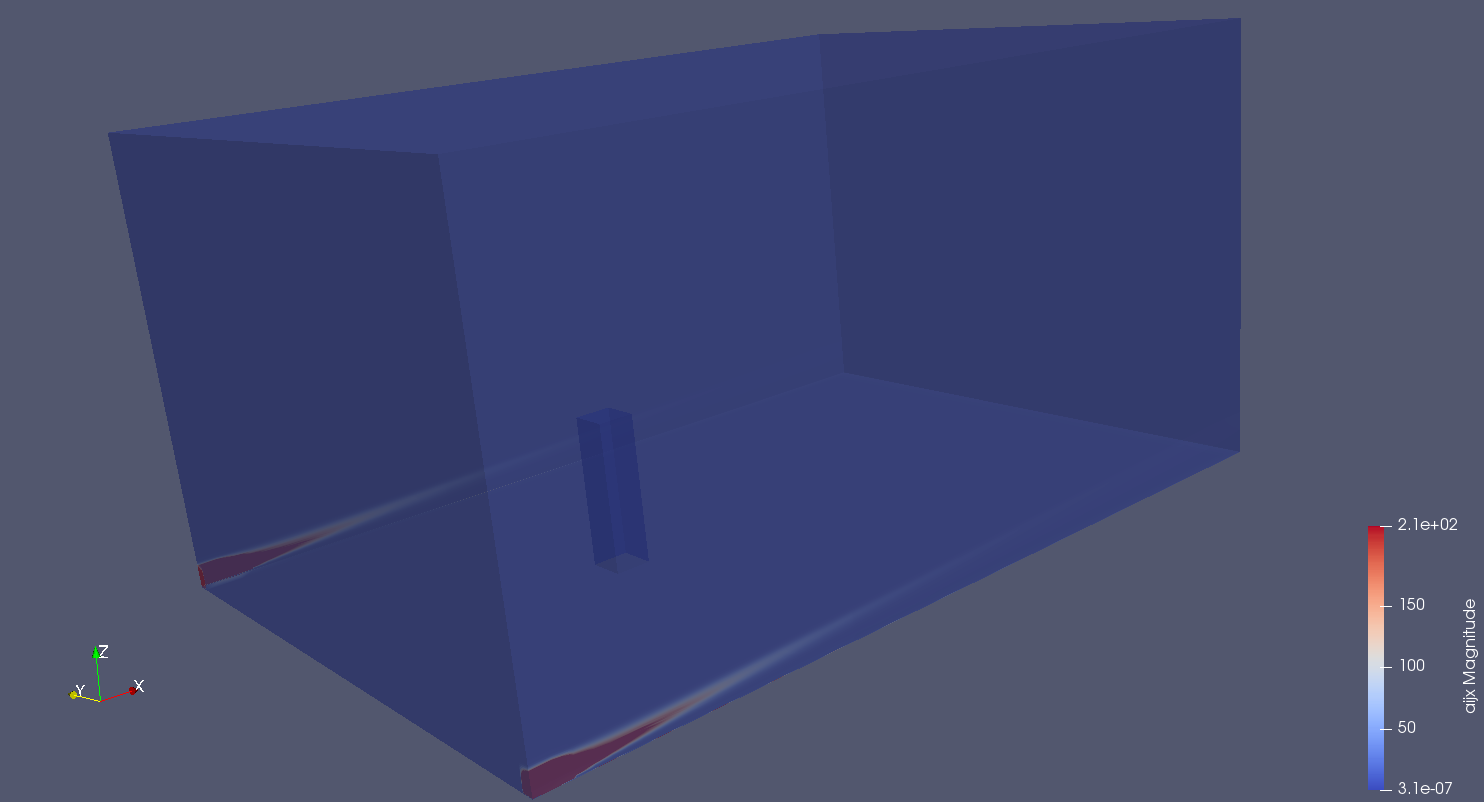
\includegraphics[width=0.45\textwidth]{figs/sqcyl/aij_magn.png}}}%
    \qquad
    \subfloat[\centering $a_{ij}^{yy}$]{{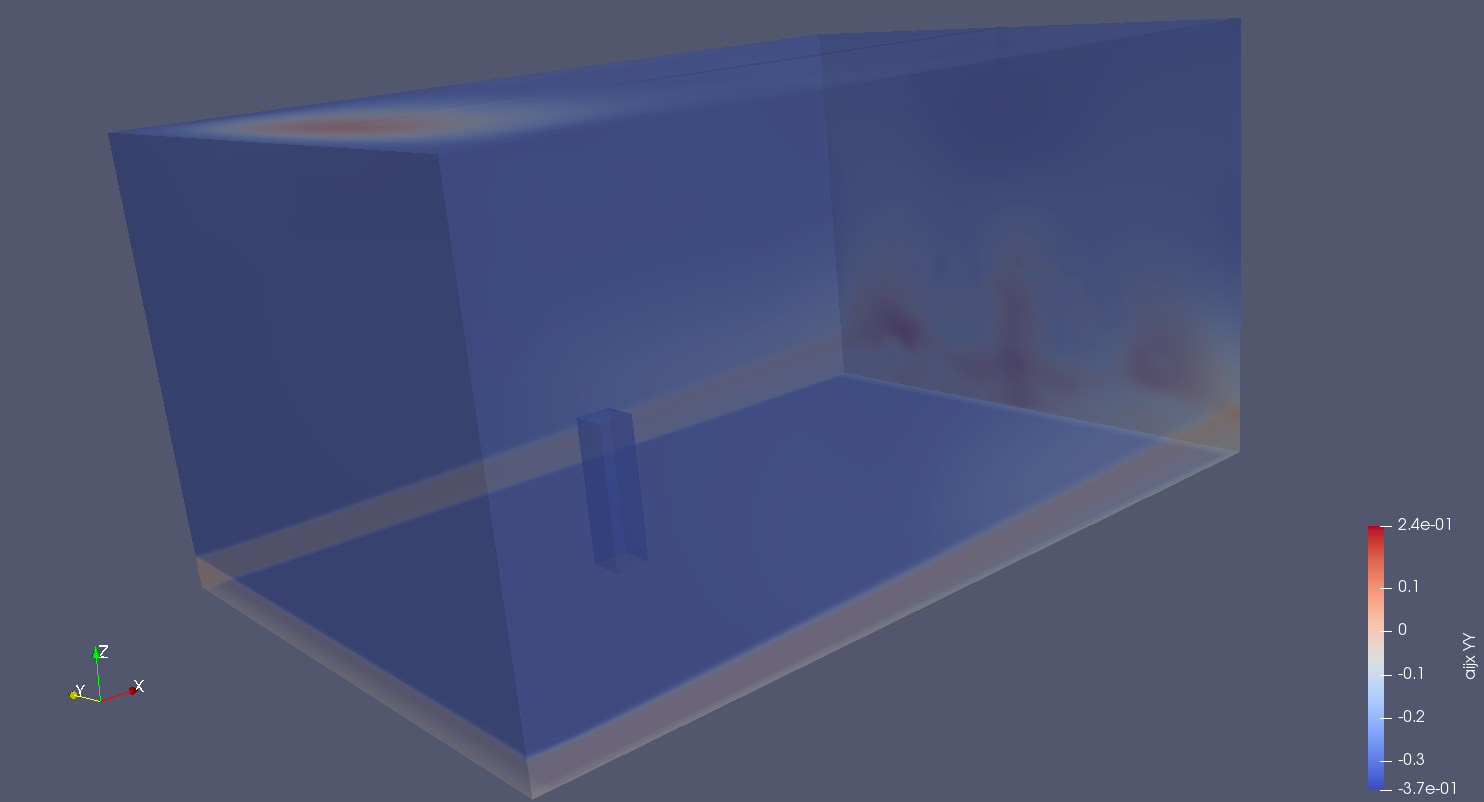
\includegraphics[width=0.45\textwidth]{figs/sqcyl/aij_yy.png}}}%
    \caption{}%
    \subfloat[\centering $k$]{{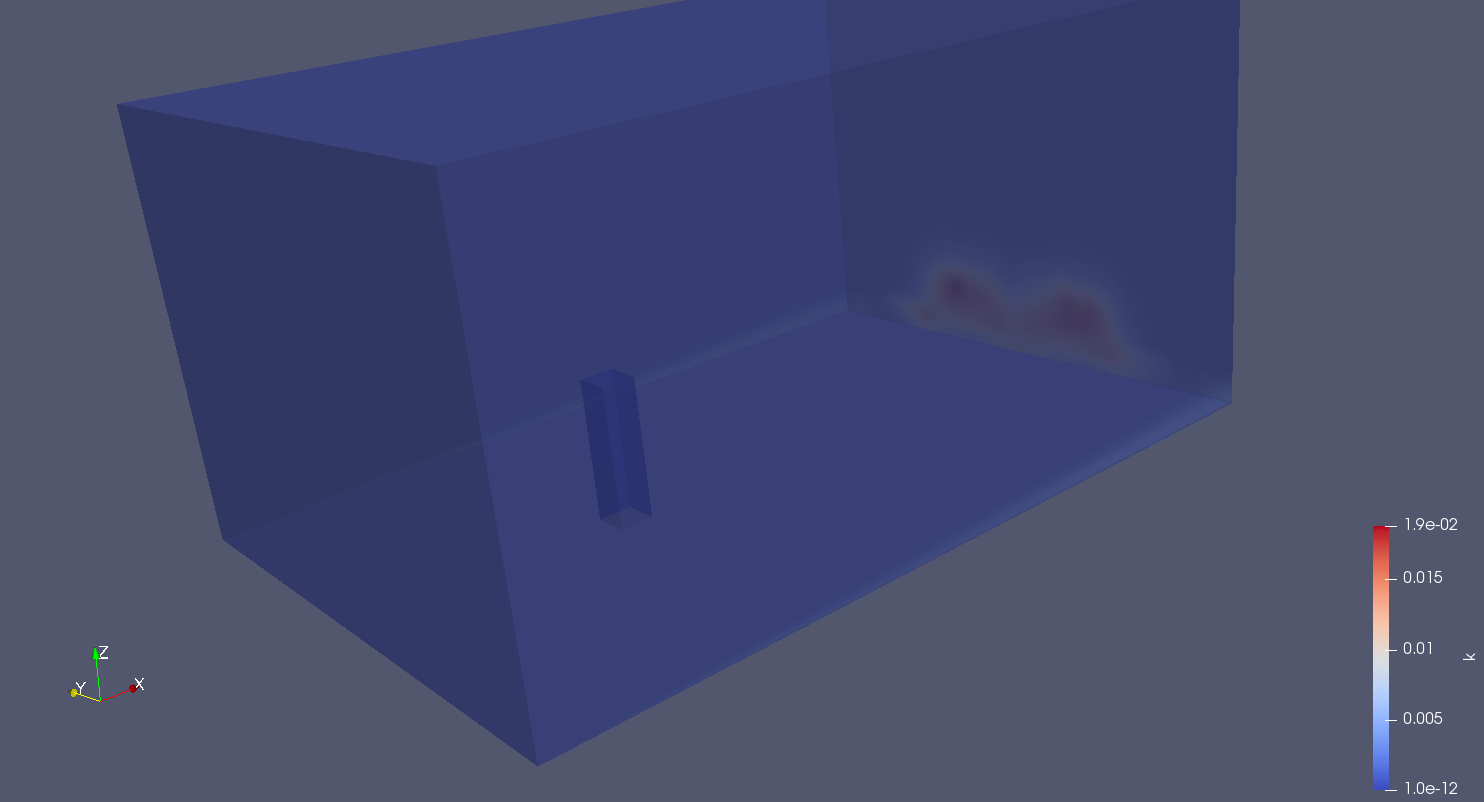
\includegraphics[width=0.45\textwidth]{figs/sqcyl/k.png}}}%
    \qquad
    \subfloat[\centering $\omega$]{{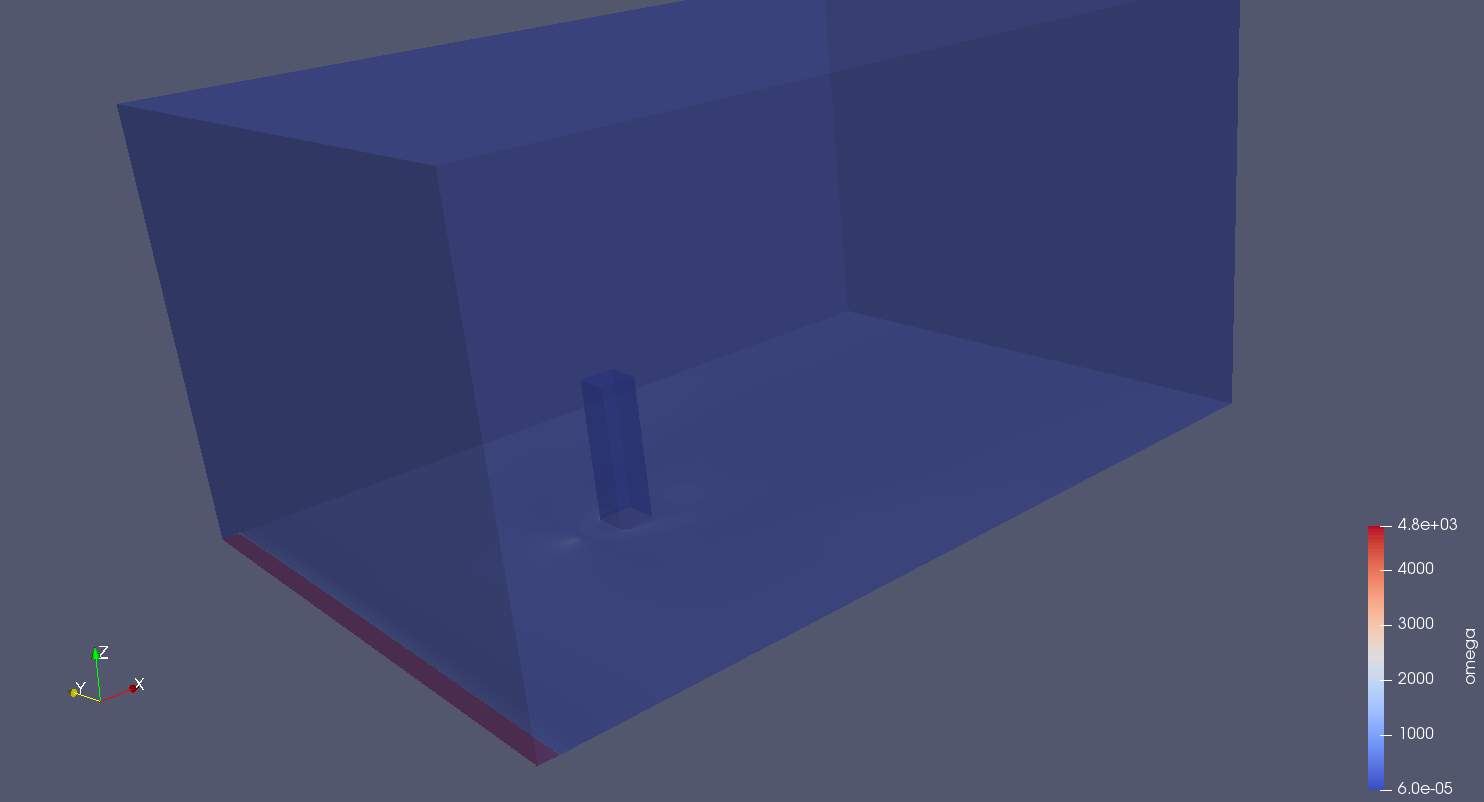
\includegraphics[width=0.45\textwidth]{figs/sqcyl/omega.png}}}%
    \caption{}%
    \subfloat[\centering $S_{ij}$ magnitude]{{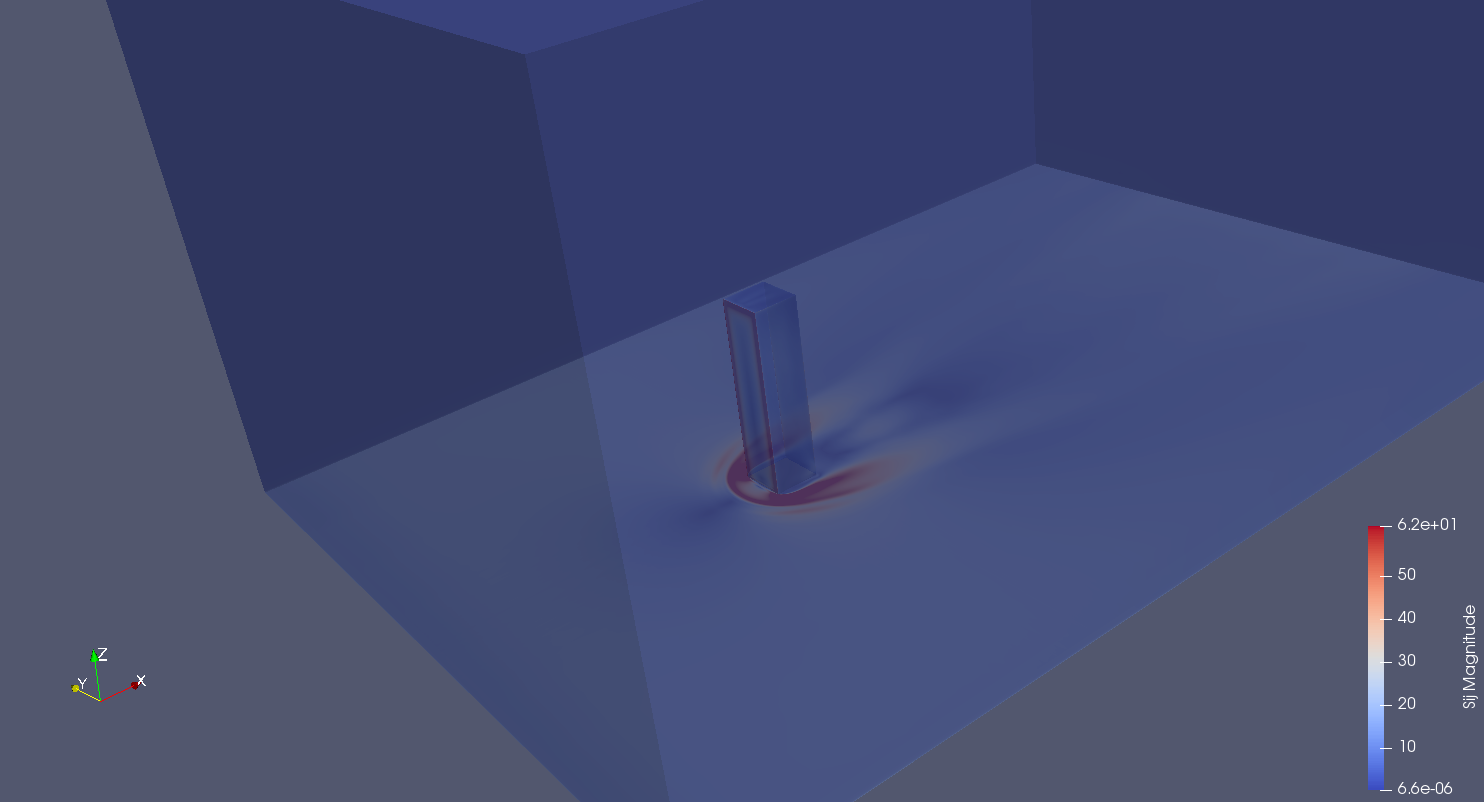
\includegraphics[width=0.45\textwidth]{figs/sqcyl/Sij.png}}}%
    \qquad
    \subfloat[\centering $\Omega_{ij}$ magnitude]{{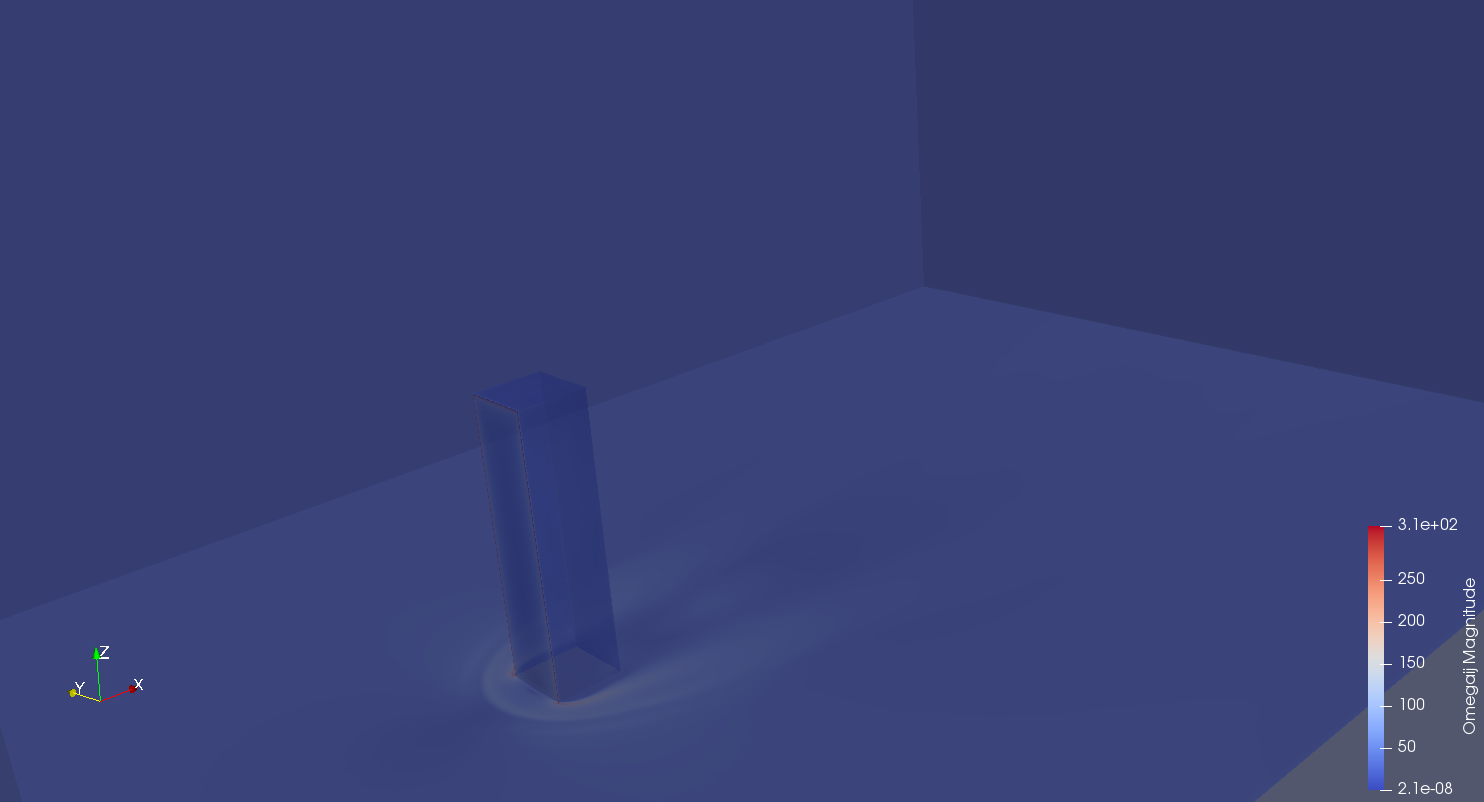
\includegraphics[width=0.45\textwidth]{figs/sqcyl/Omegaij.png}}}%
    \caption{}%
    \label{fig:sqcyl}%
\end{figure}

\begin{figure}[H]%
    \centering
    \subfloat[\centering $b_{ij}$ magnitude]{{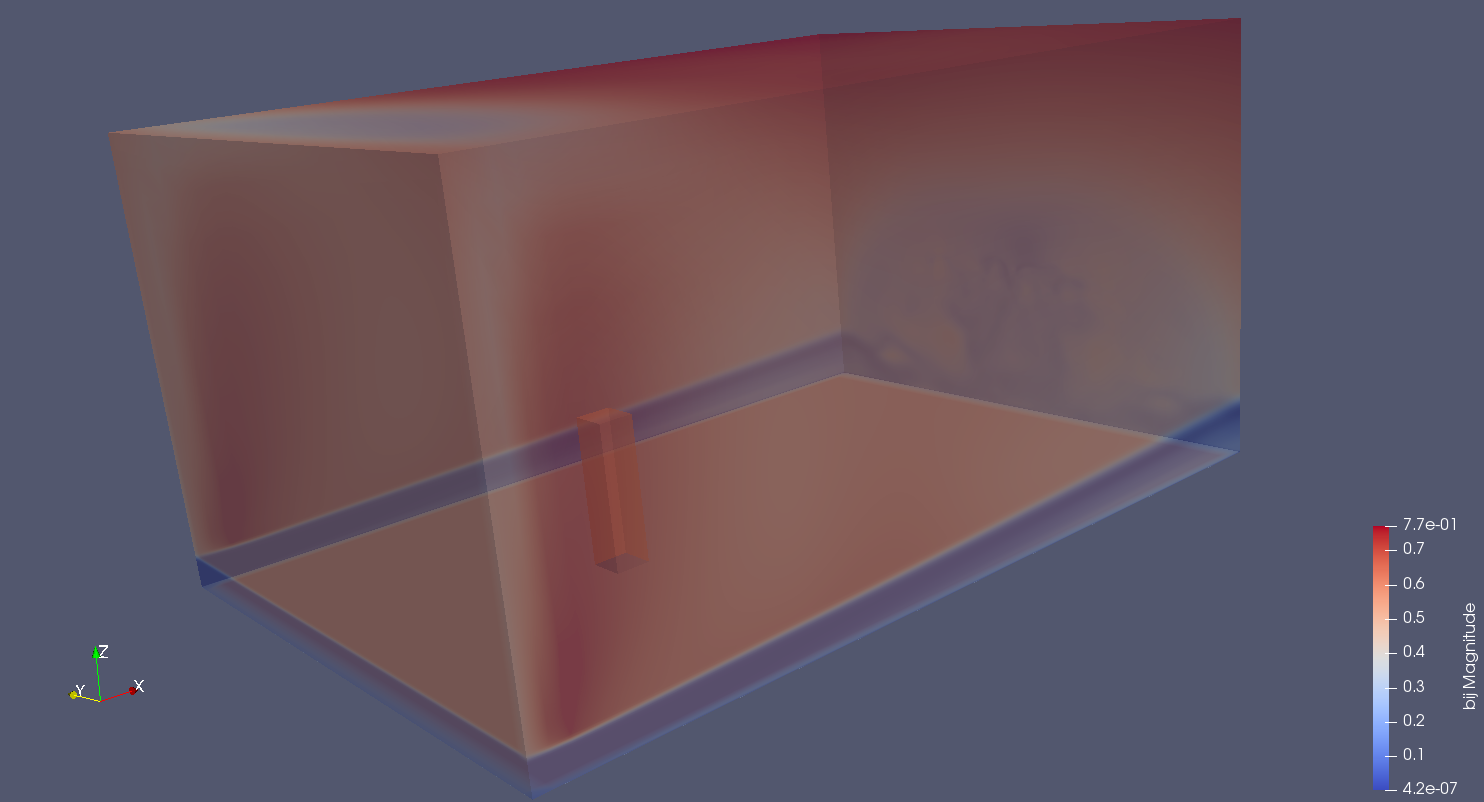
\includegraphics[width=0.45\textwidth]{figs/sqcyl/bij_magn.png}}}%
    \qquad
    \subfloat[\centering $b_{ij}^{xx}$]{{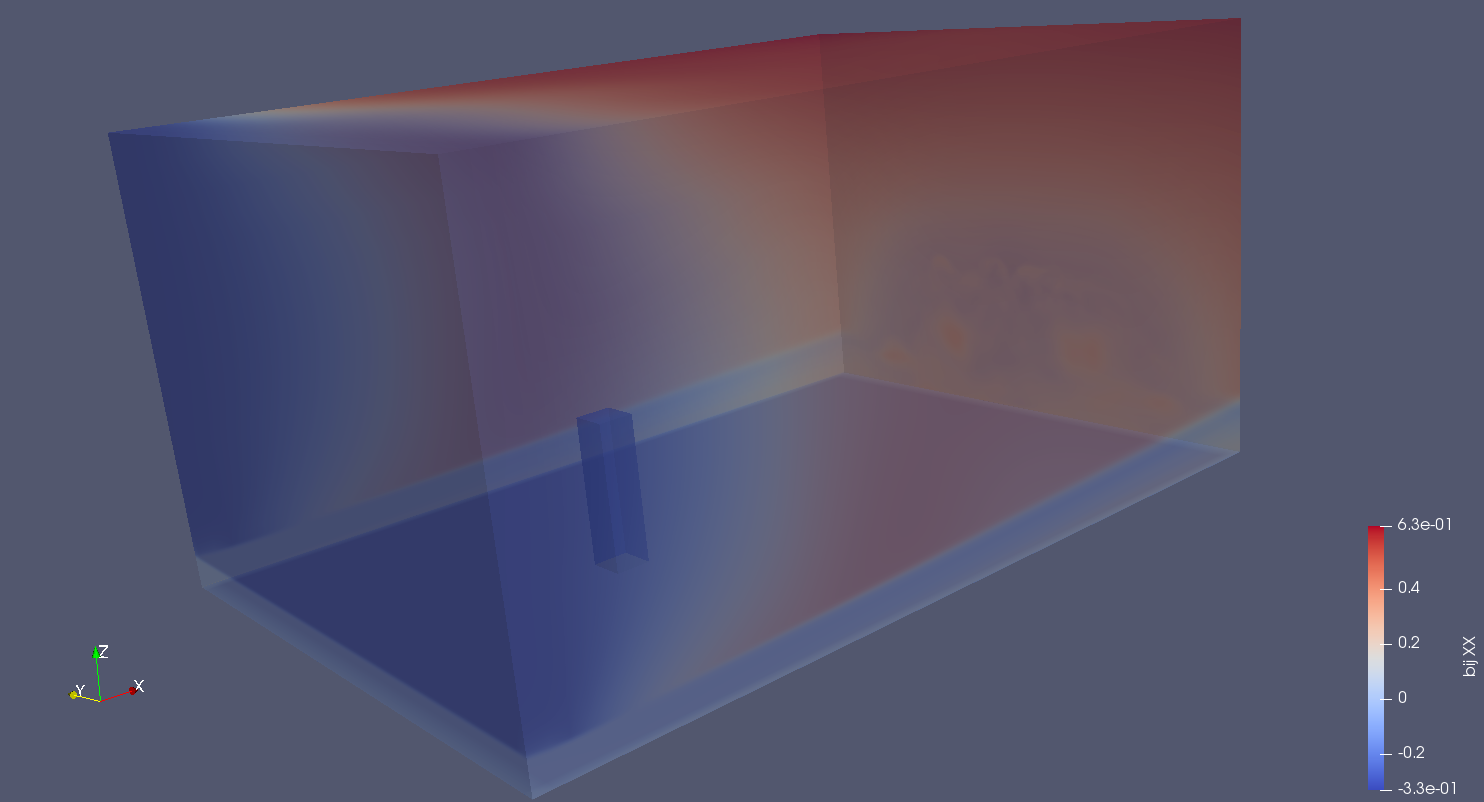
\includegraphics[width=0.45\textwidth]{figs/sqcyl/bij_xx.png}}}%
    \caption{}%
    \subfloat[\centering $b_{ij}^{xy}$]{{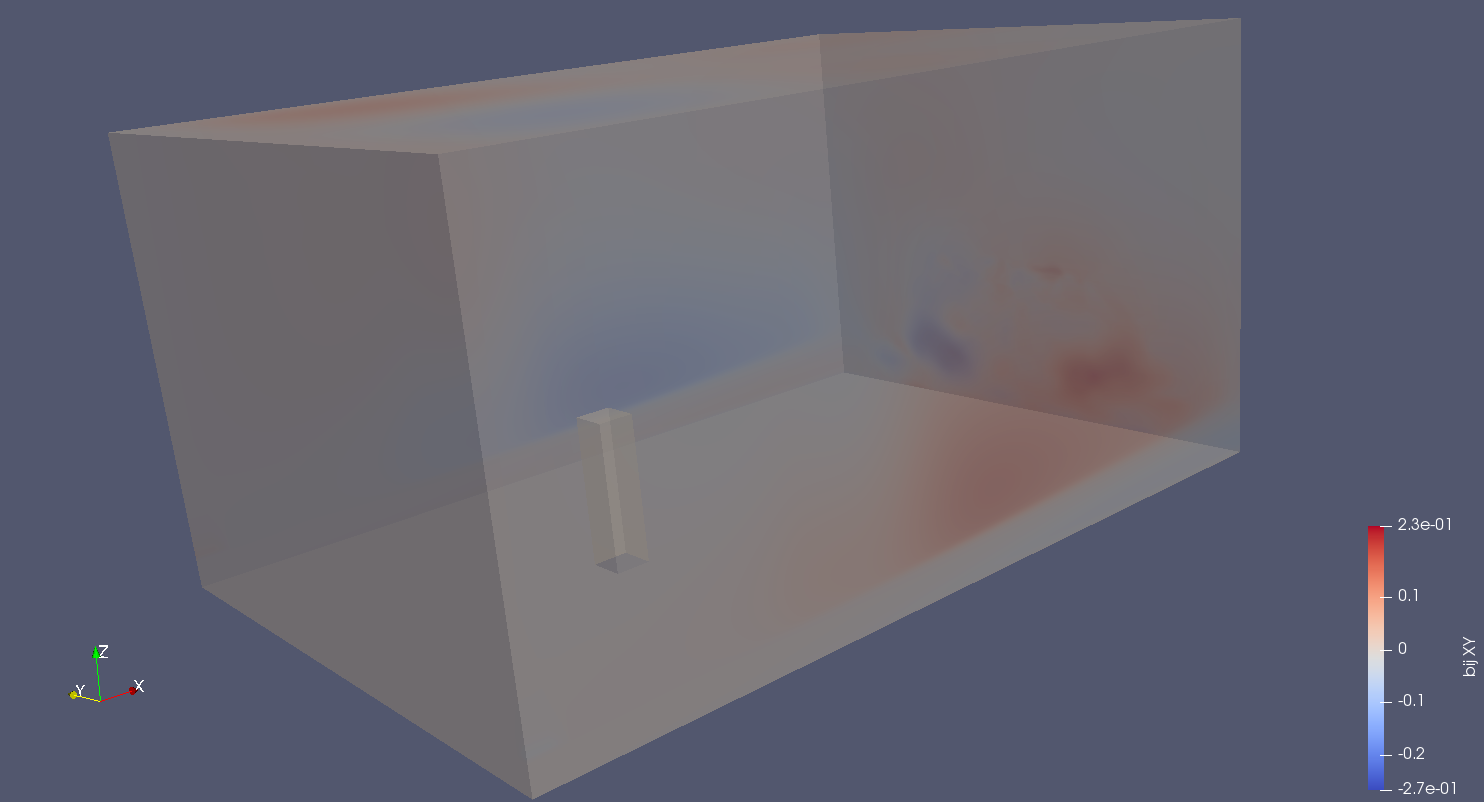
\includegraphics[width=0.45\textwidth]{figs/sqcyl/bij_xy.png}}}%
    \qquad
    \subfloat[\centering $b_{ij}^{xz}$]{{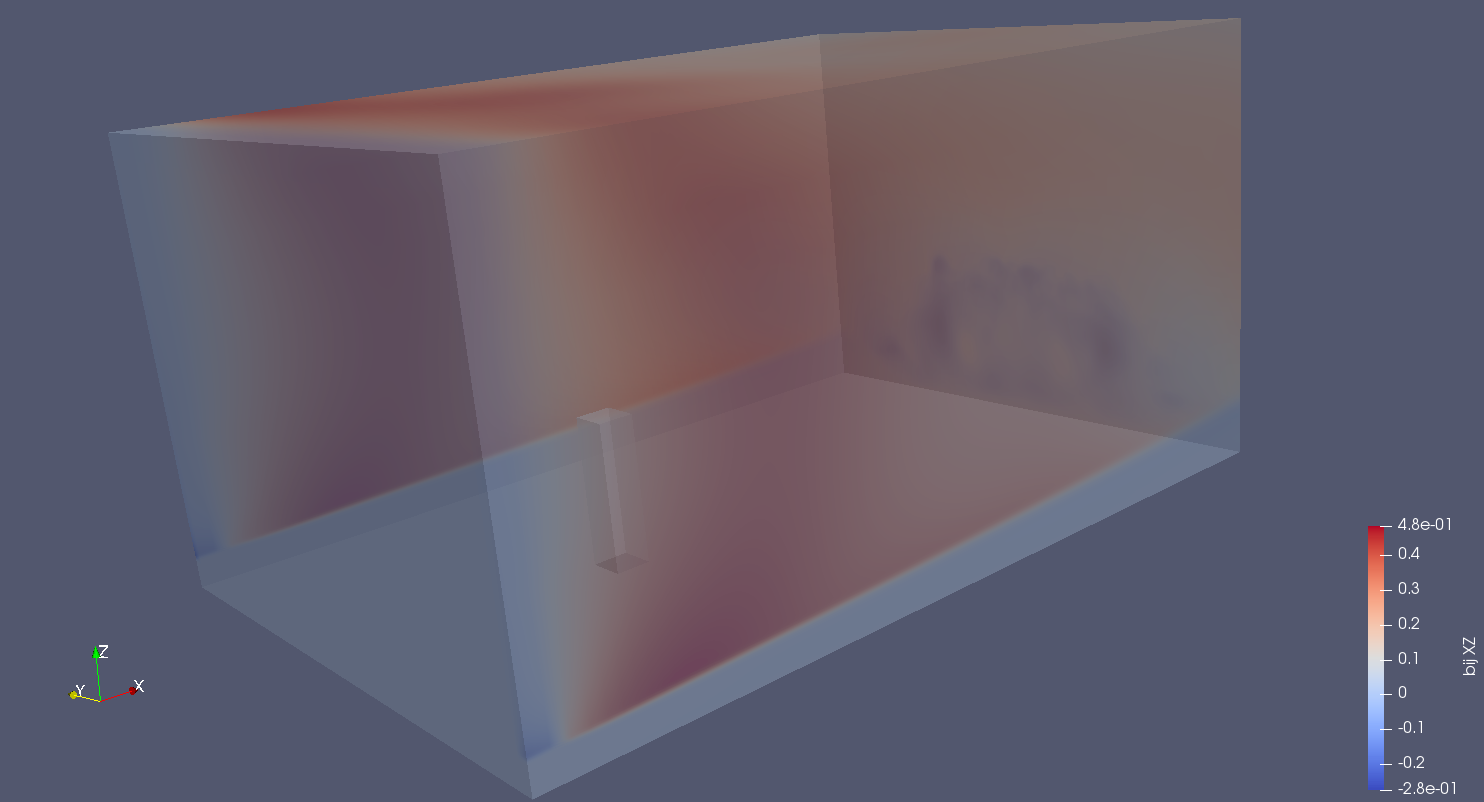
\includegraphics[width=0.45\textwidth]{figs/sqcyl/bij_xz.png}}}%
    \caption{}%
    \subfloat[\centering $b_{ij}^{yy}$]{{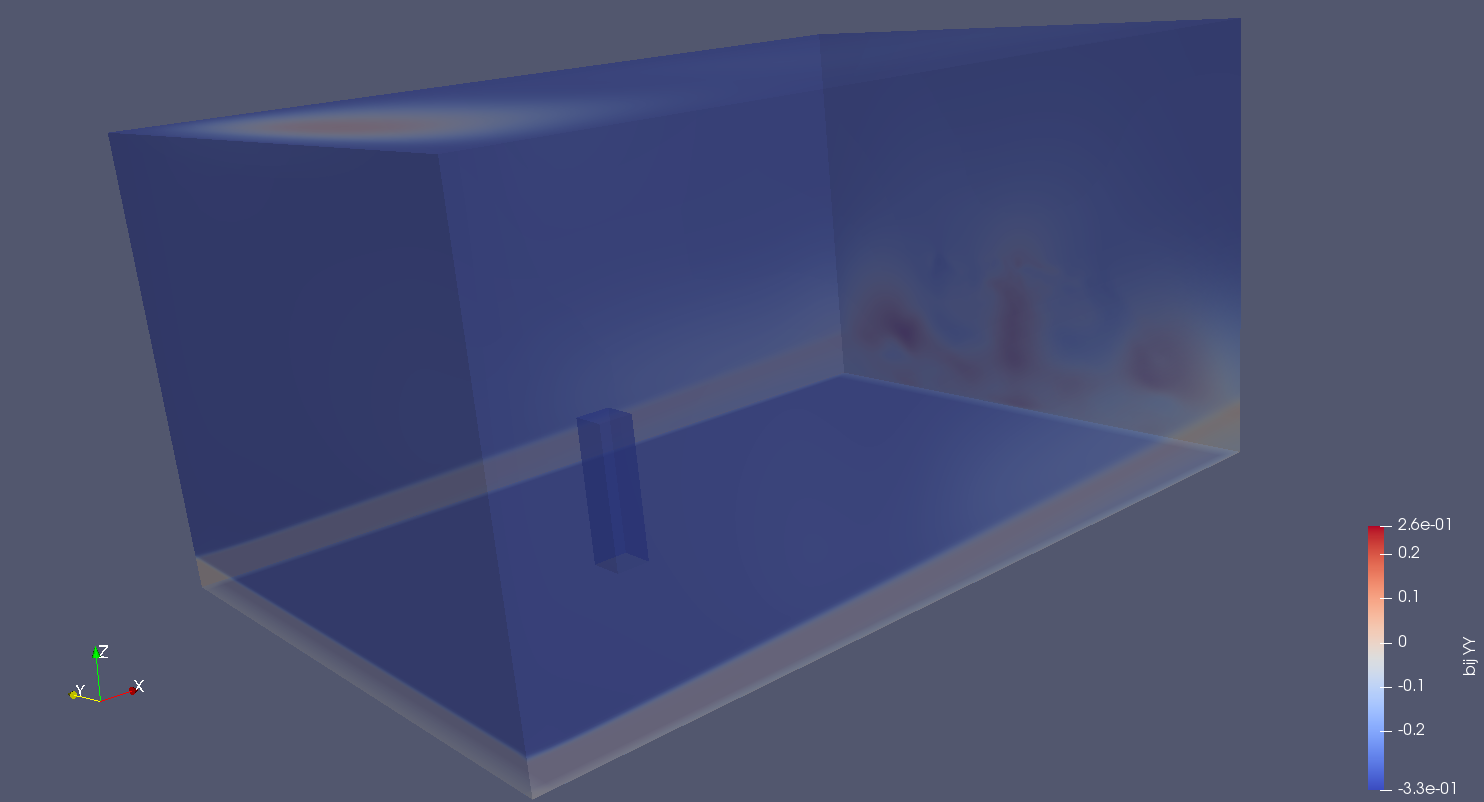
\includegraphics[width=0.45\textwidth]{figs/sqcyl/bij_yy.png}}}%
    \qquad
    \subfloat[\centering $b_{ij}^{yz}$]{{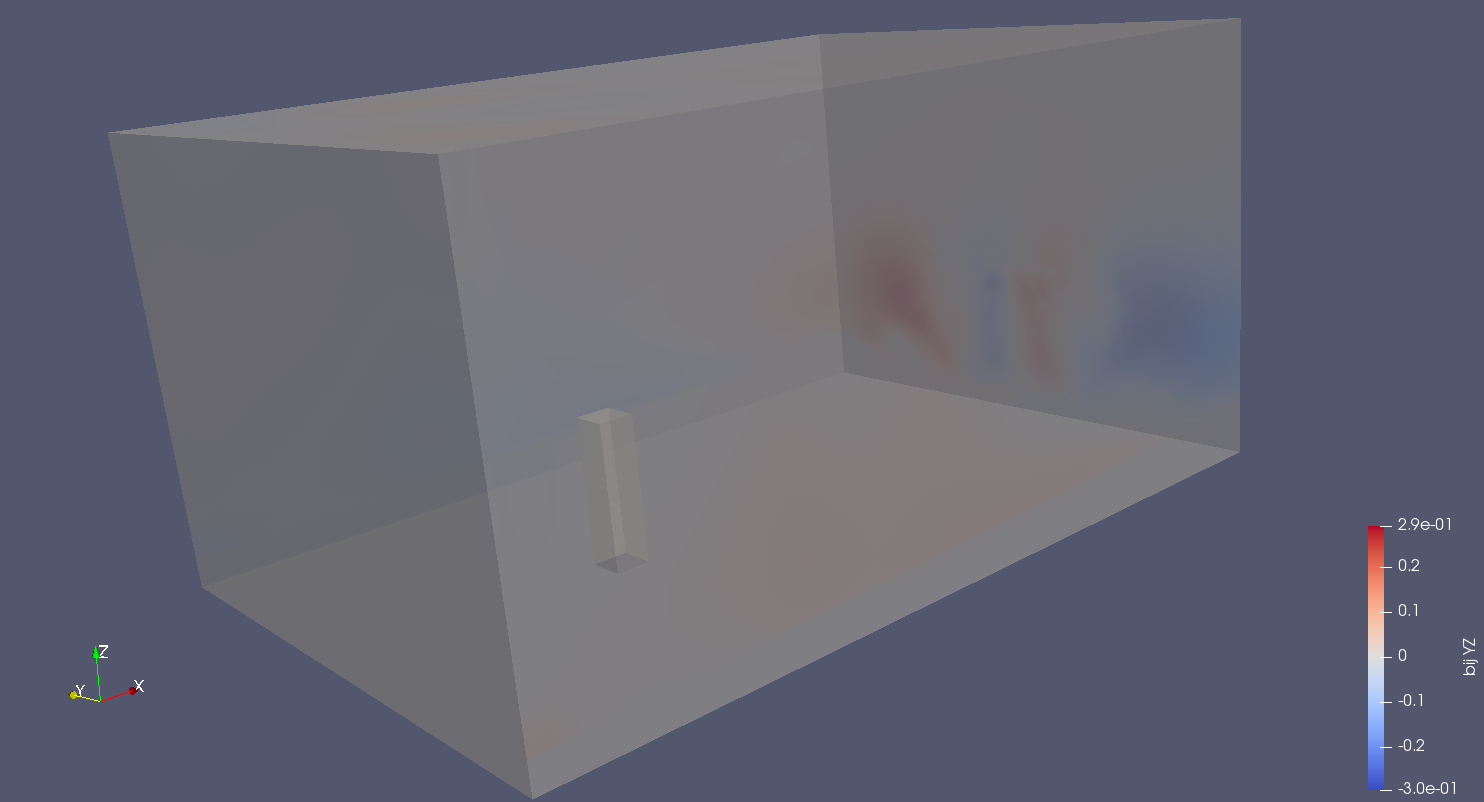
\includegraphics[width=0.45\textwidth]{figs/sqcyl/bij_yz.png}}}%
    \caption{}%
    \subfloat[\centering $b_{ij}^{zz}$]{{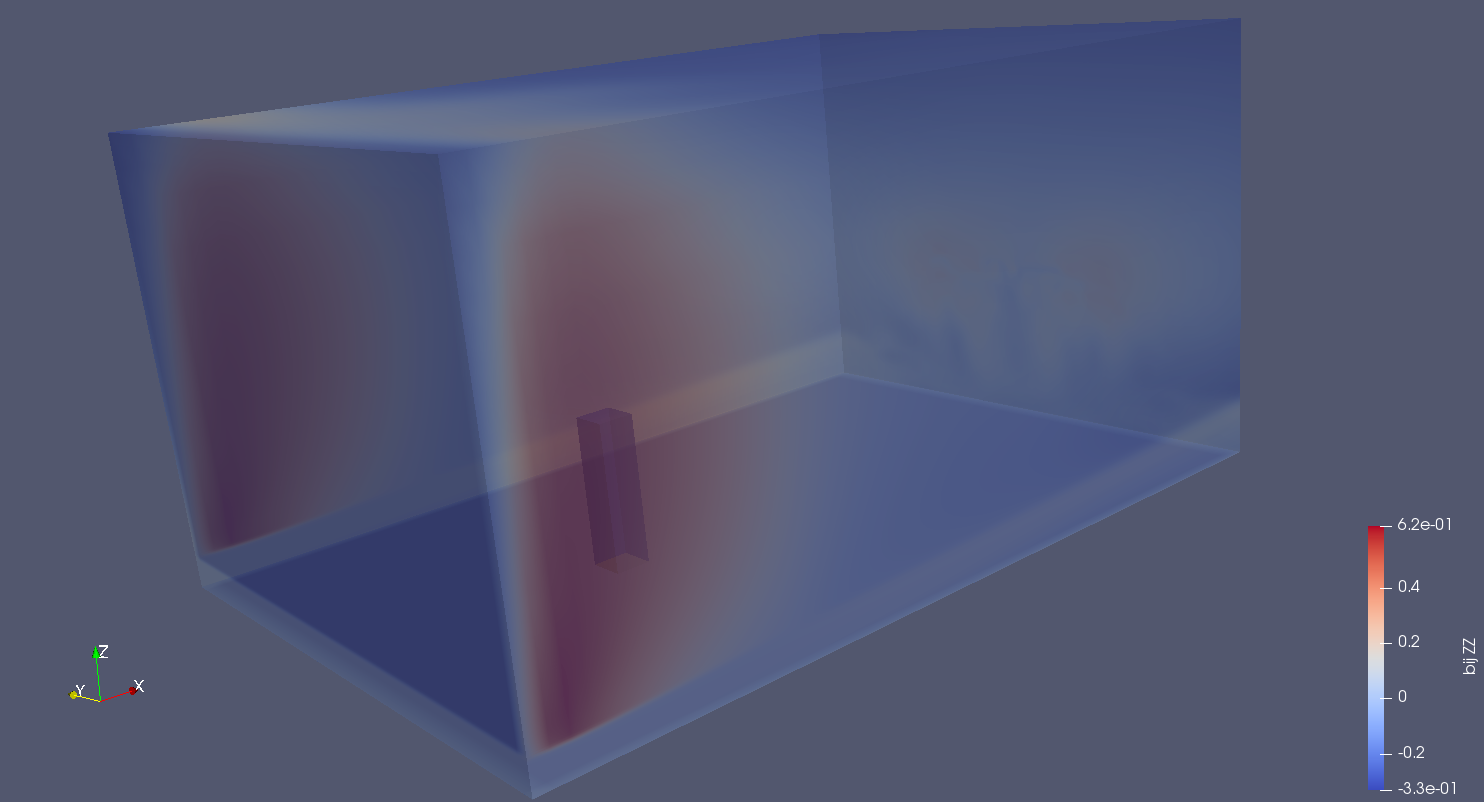
\includegraphics[width=0.45\textwidth]{figs/sqcyl/bij_zz.png}}}%
    \qquad
    \subfloat[\centering $\nu_t$]{{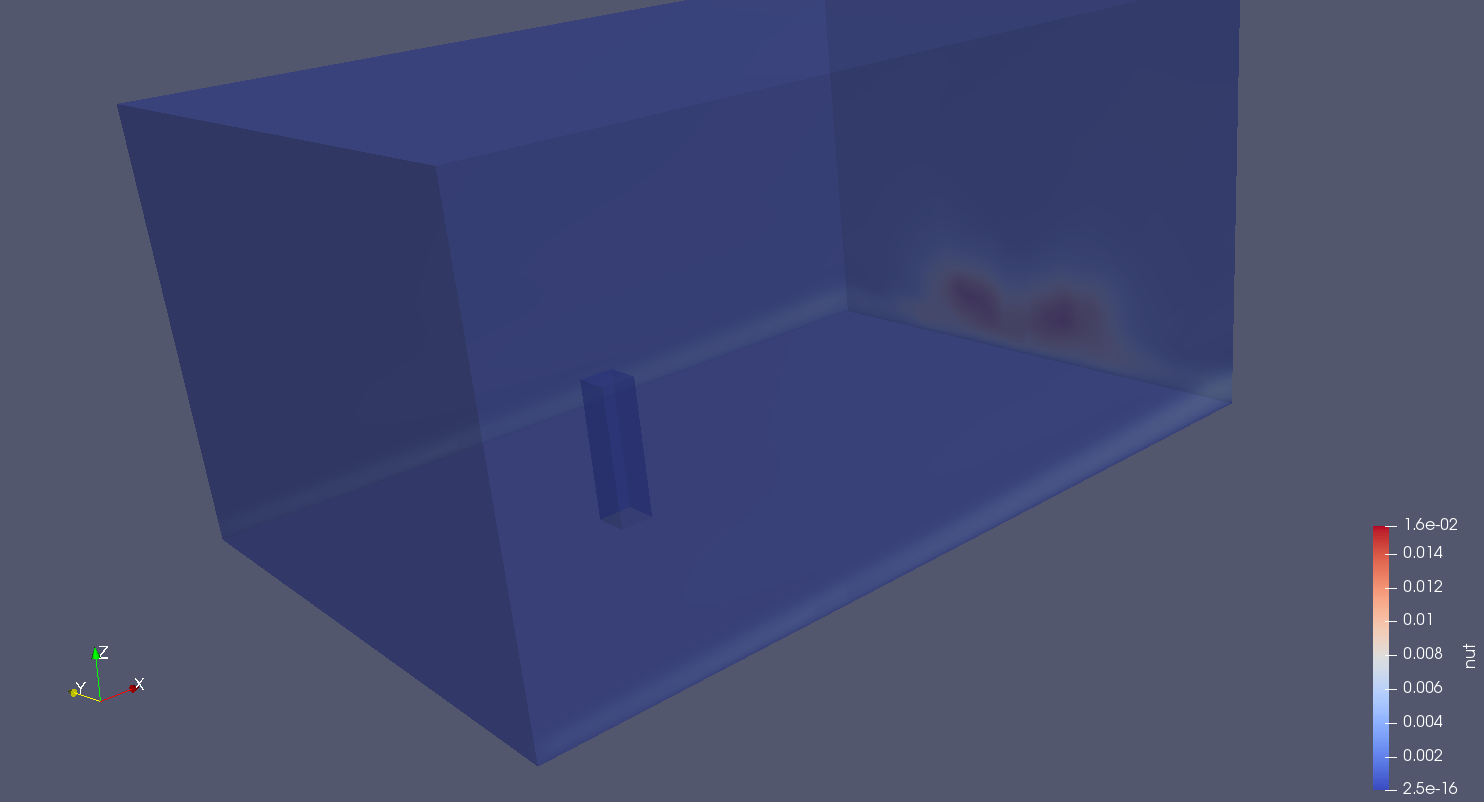
\includegraphics[width=0.45\textwidth]{figs/sqcyl/nut.png}}}%
    \caption{}%
    \label{fig:sqcyl}%
\end{figure}

\begin{figure}[H]%
    \centering
    \subfloat[\centering $I_1$]{{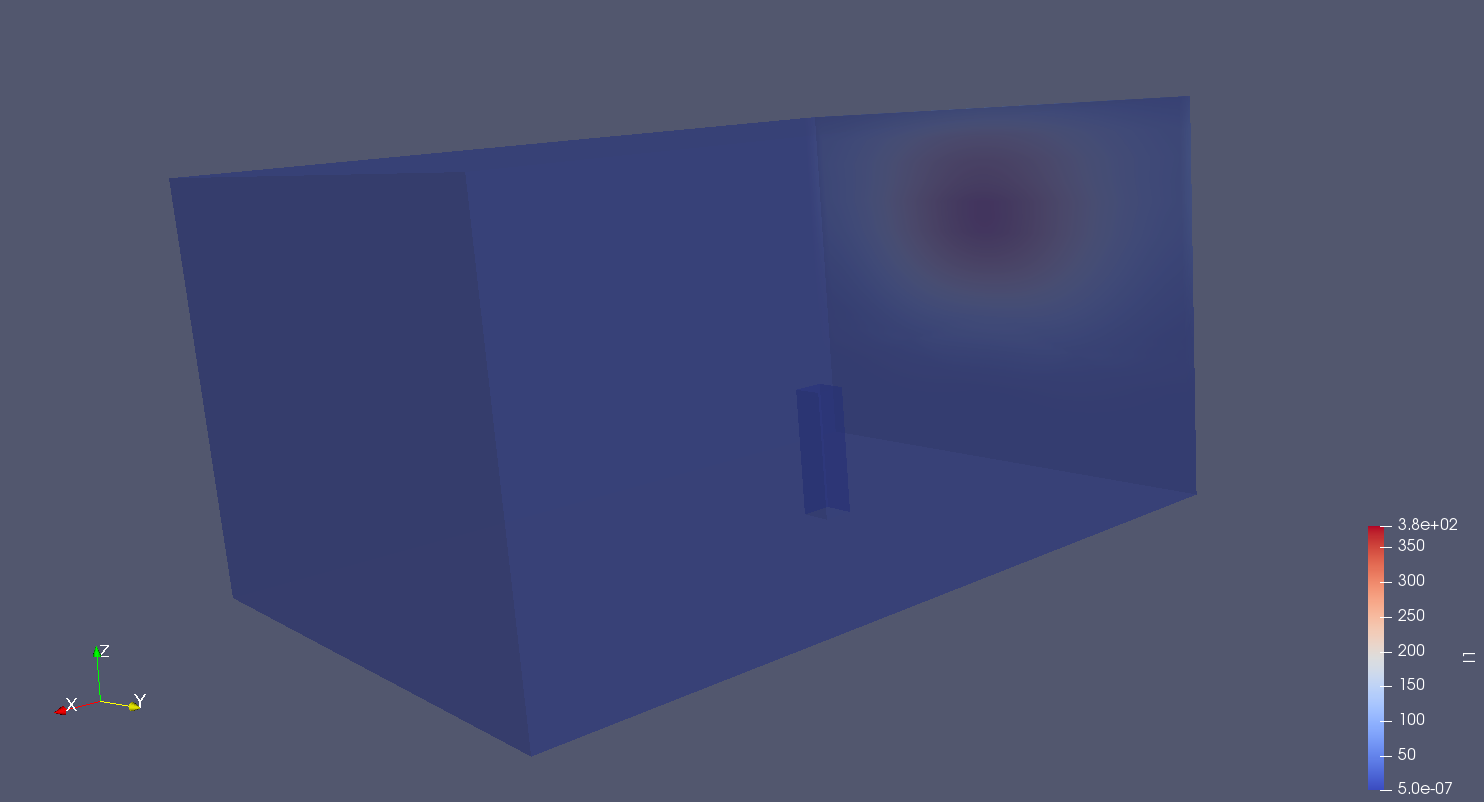
\includegraphics[width=0.45\textwidth]{figs/sqcyl/I1.png}}}%
    \qquad
    \subfloat[\centering $R$ term]{{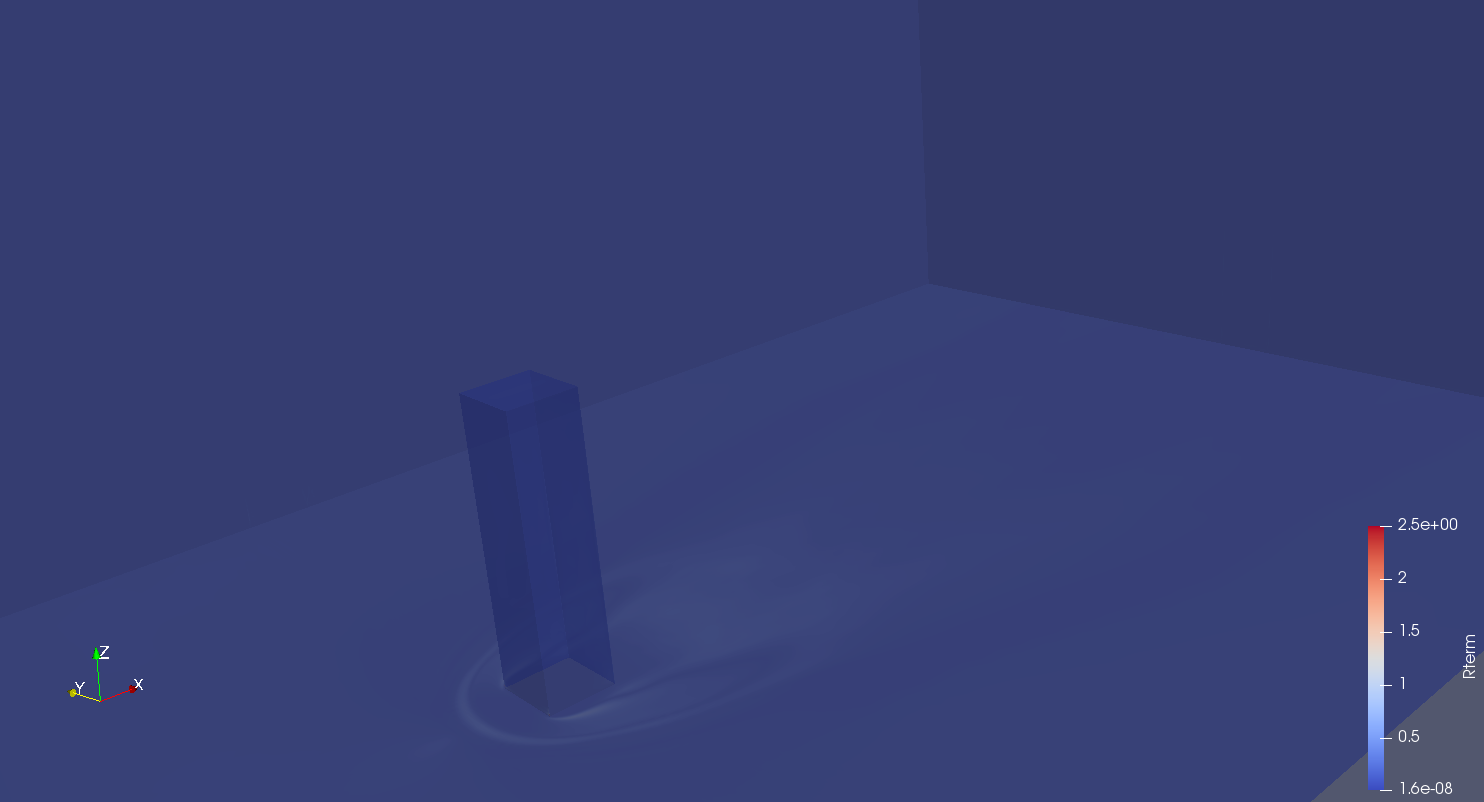
\includegraphics[width=0.45\textwidth]{figs/sqcyl/Rterm.png}}}%
    \caption{}%
    \subfloat[\centering $R$ term norm]{{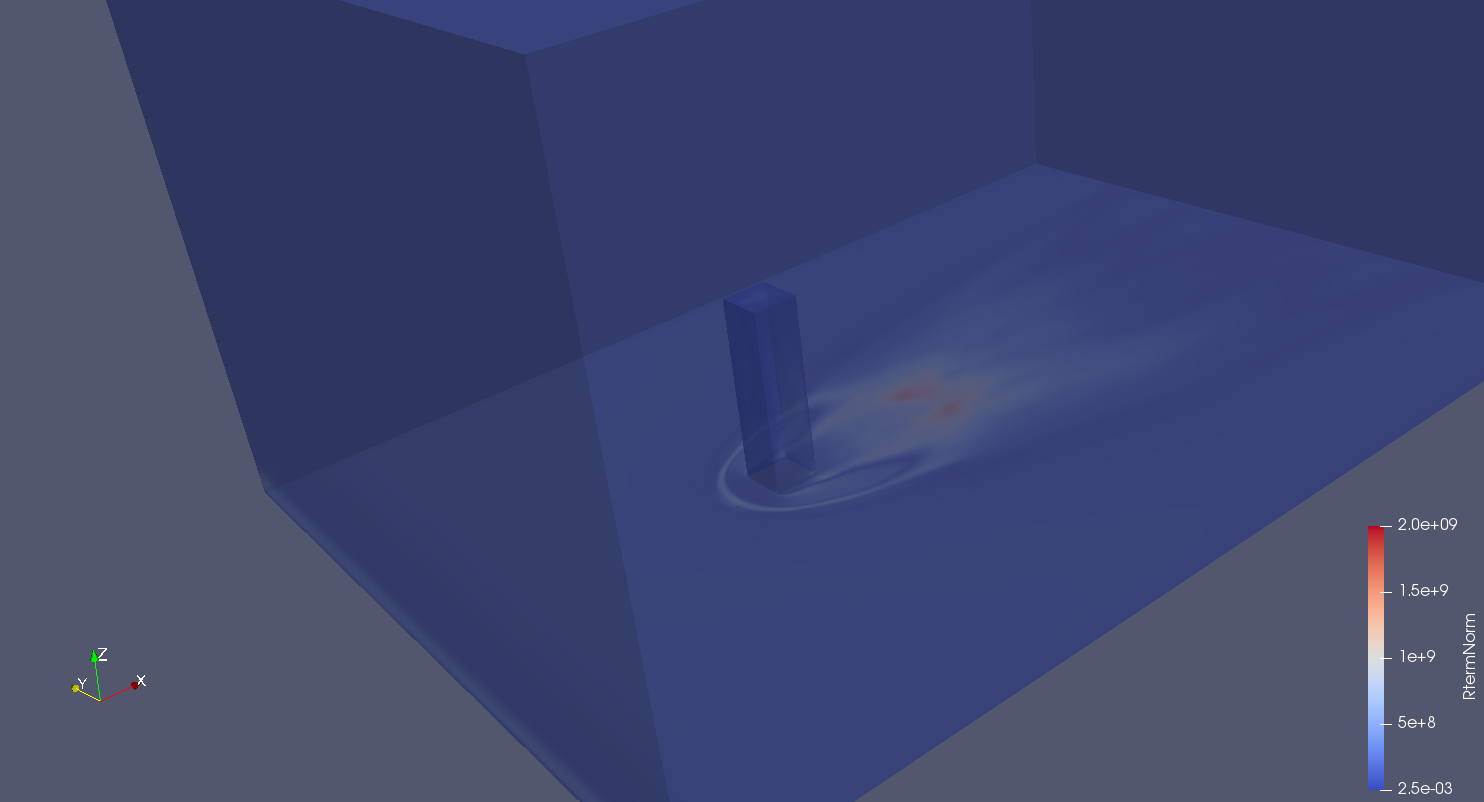
\includegraphics[width=0.45\textwidth]{figs/sqcyl/RtermNorm.png}}}%
    \qquad
    \subfloat[\centering $T_1$ magnitude]{{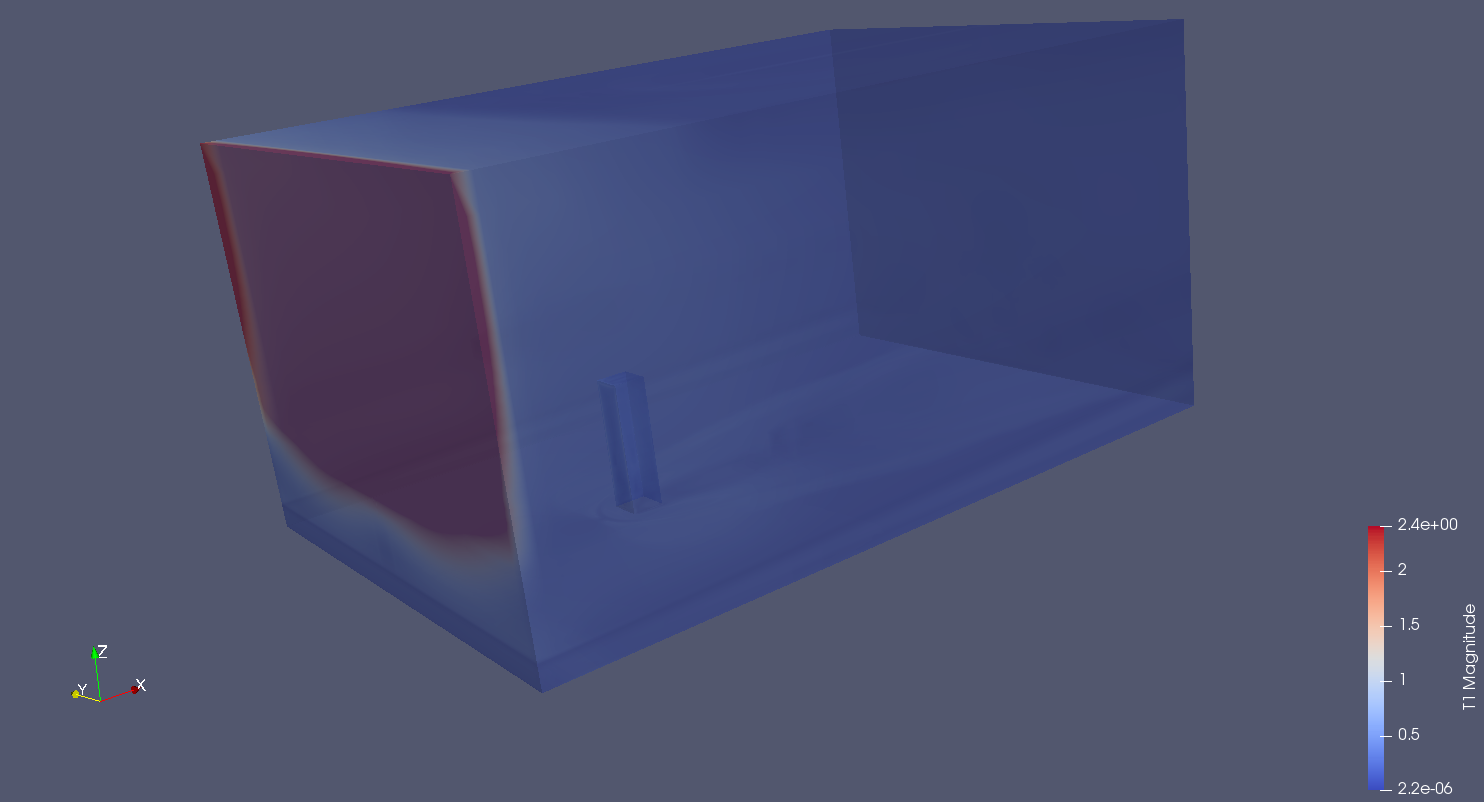
\includegraphics[width=0.45\textwidth]{figs/sqcyl/T1_magn.png}}}%
    \caption{}%
    \subfloat[\centering $T_2$ magnitude]{{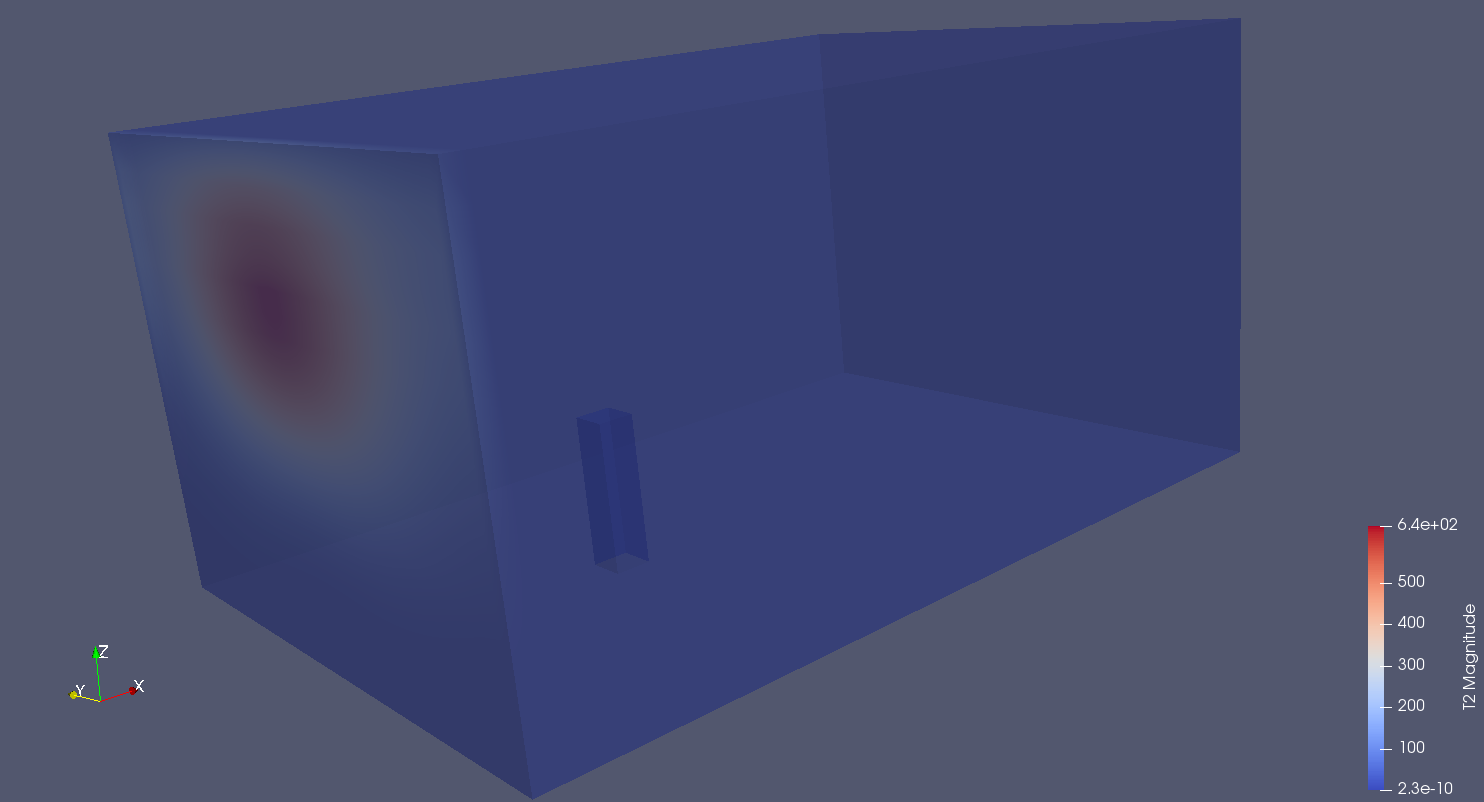
\includegraphics[width=0.45\textwidth]{figs/sqcyl/T2_magn.png}}}%
    \qquad
    \subfloat[\centering $R_{res}$]{{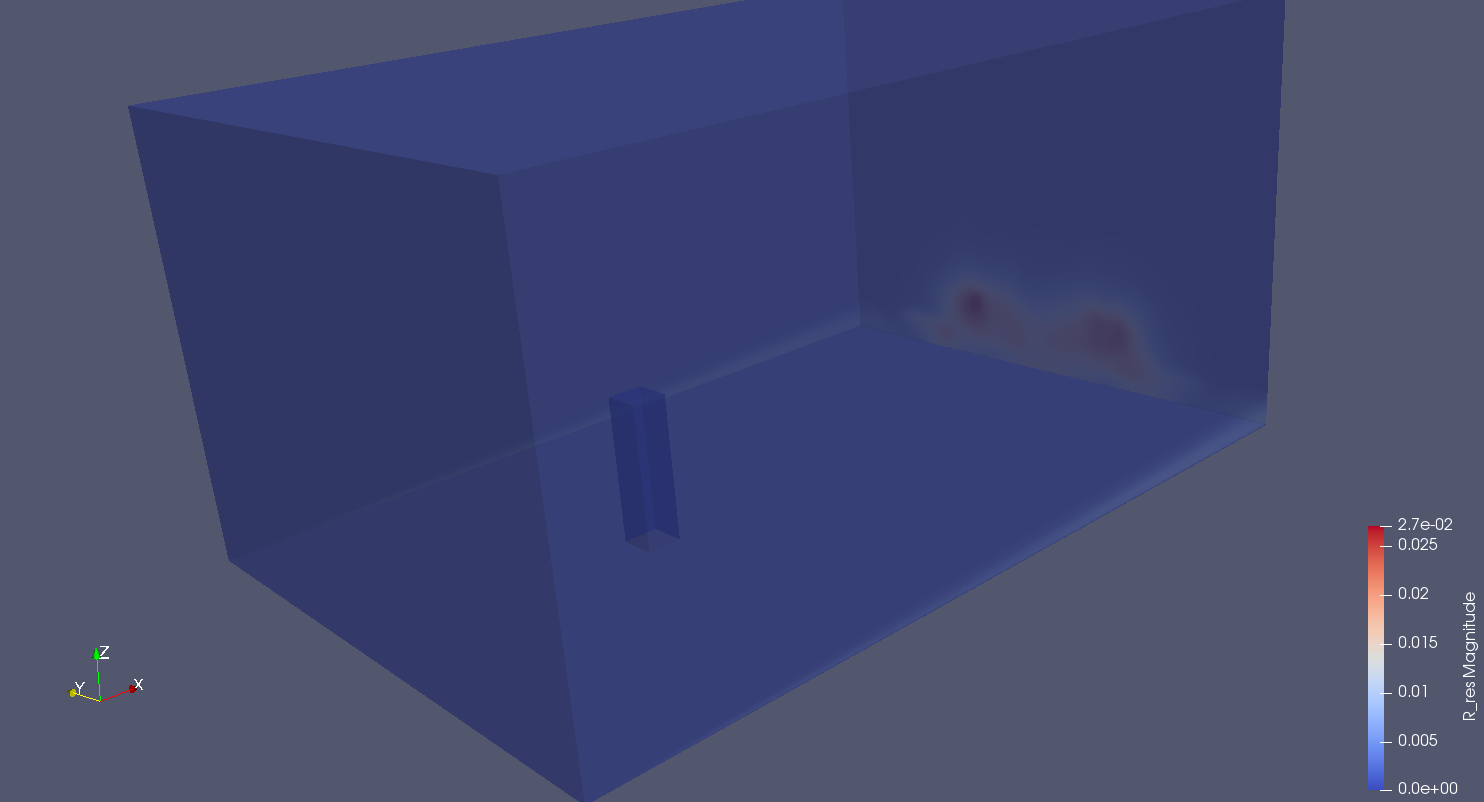
\includegraphics[width=0.45\textwidth]{figs/sqcyl/R_res.png}}}%
    \caption{}%
    \subfloat[\centering $R_{sgs}$]{{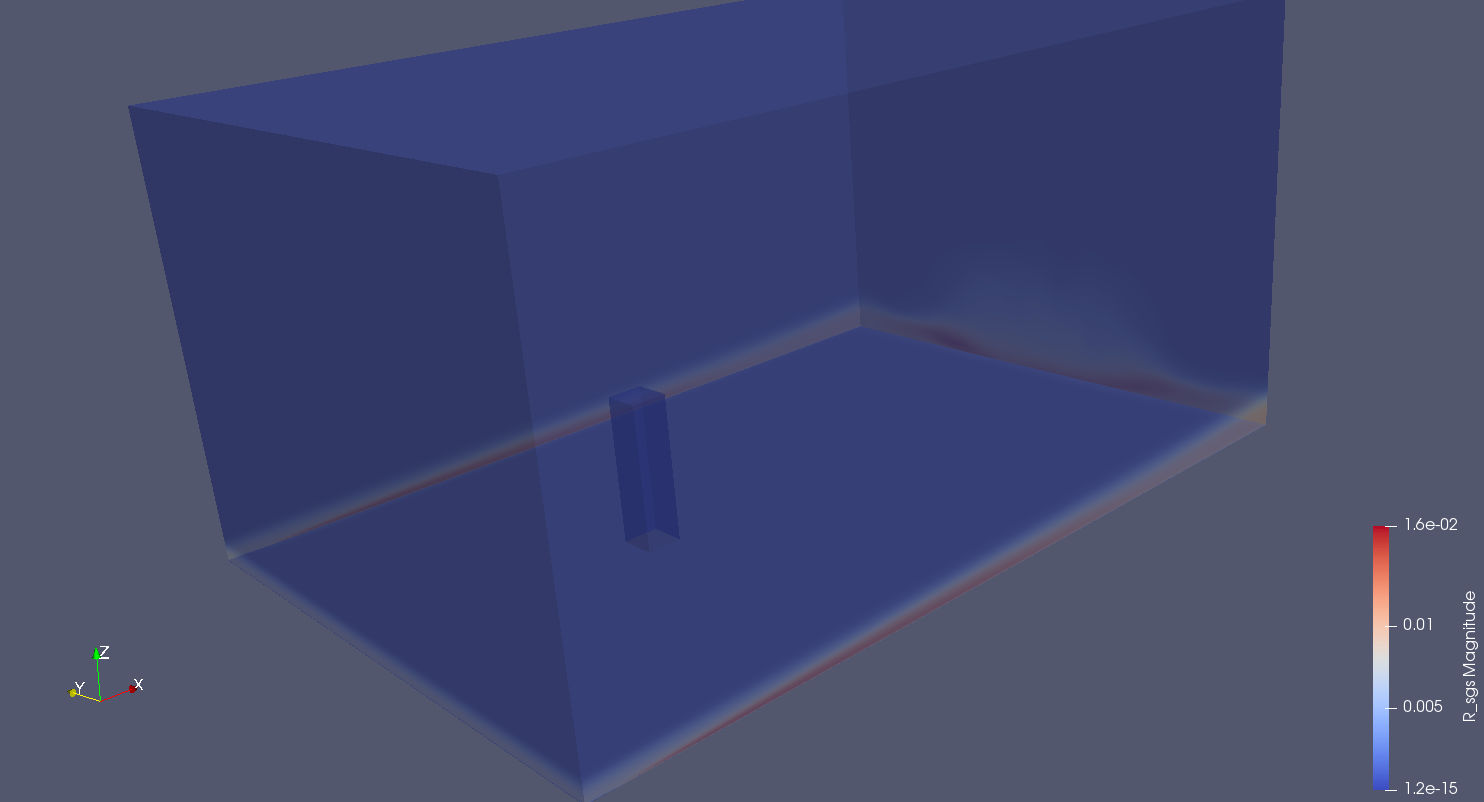
\includegraphics[width=0.45\textwidth]{figs/sqcyl/R_sgs.png}}}%
    \qquad
    \subfloat[\centering $R_{tot}$]{{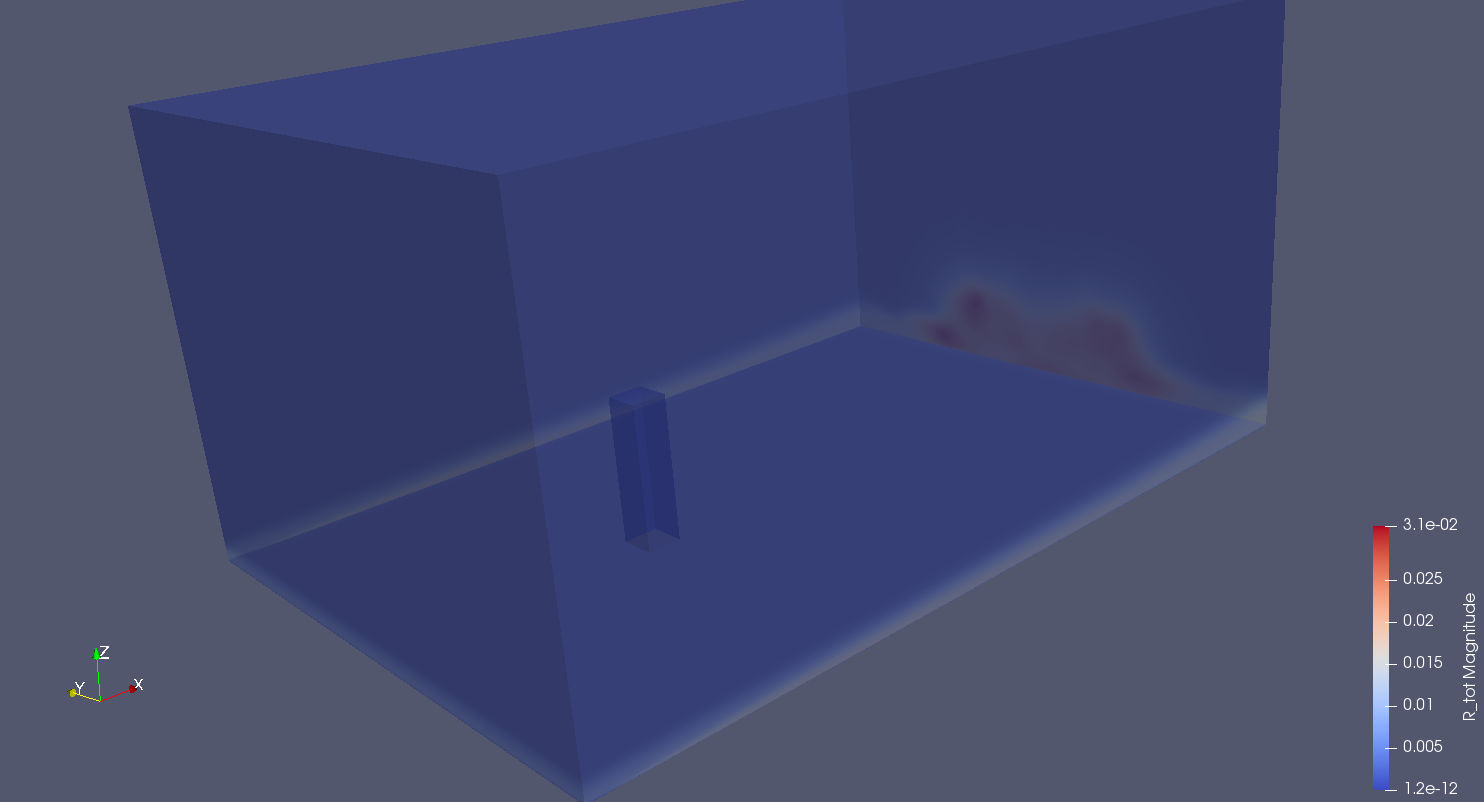
\includegraphics[width=0.45\textwidth]{figs/sqcyl/R_tot.png}}}%
    \caption{Some fields for a wall-mounted squared cylinder testcase.}%
    \label{fig:sqcyl}%
\end{figure}

\begin{figure}[H]%
    \centering
    \subfloat[\centering OF]{{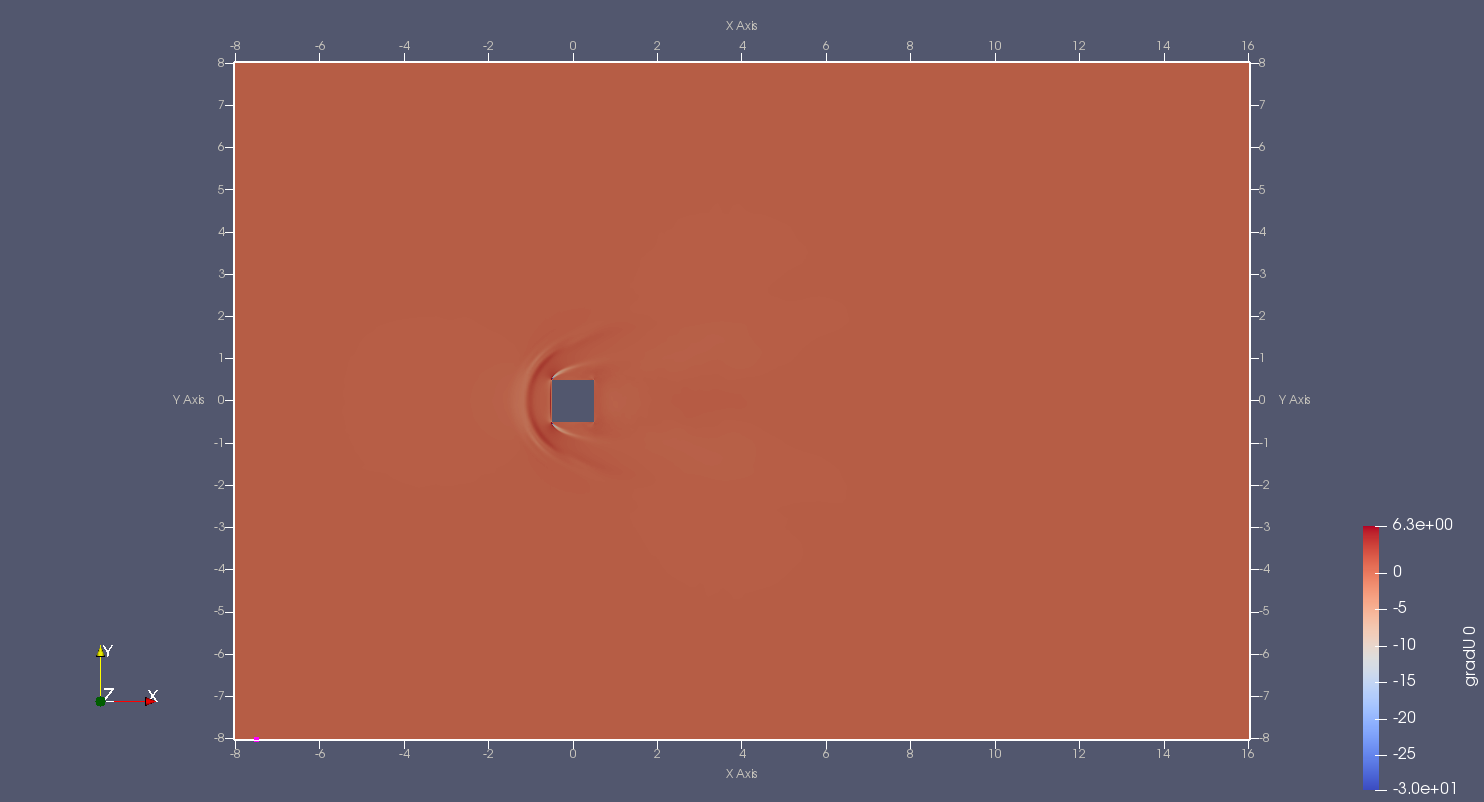
\includegraphics[width=0.45\textwidth]{figs/sqcyl/gradU/gradU0.png}}}%
    \qquad
    \subfloat[\centering R]{{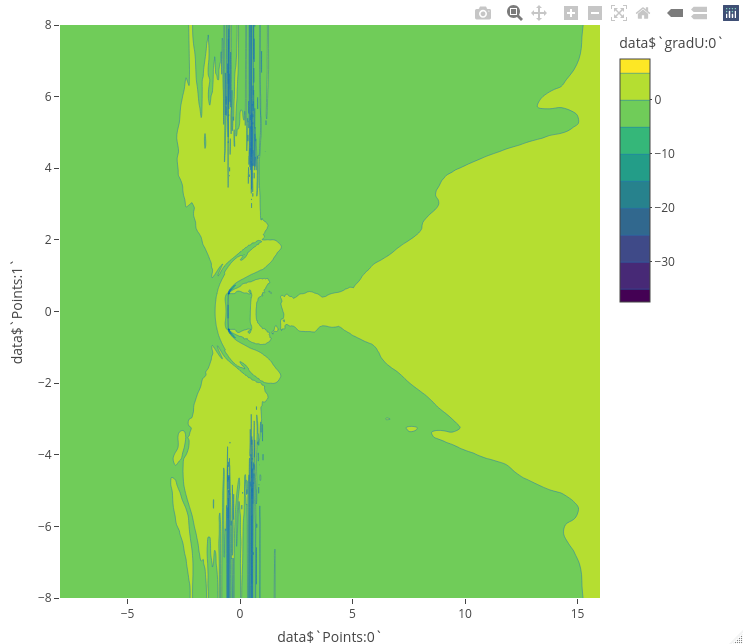
\includegraphics[width=0.3\textwidth]{figs/sqcyl/gradU_R/gradU0.png}}}%
    \caption{gradU0}%
    \subfloat[\centering OF]{{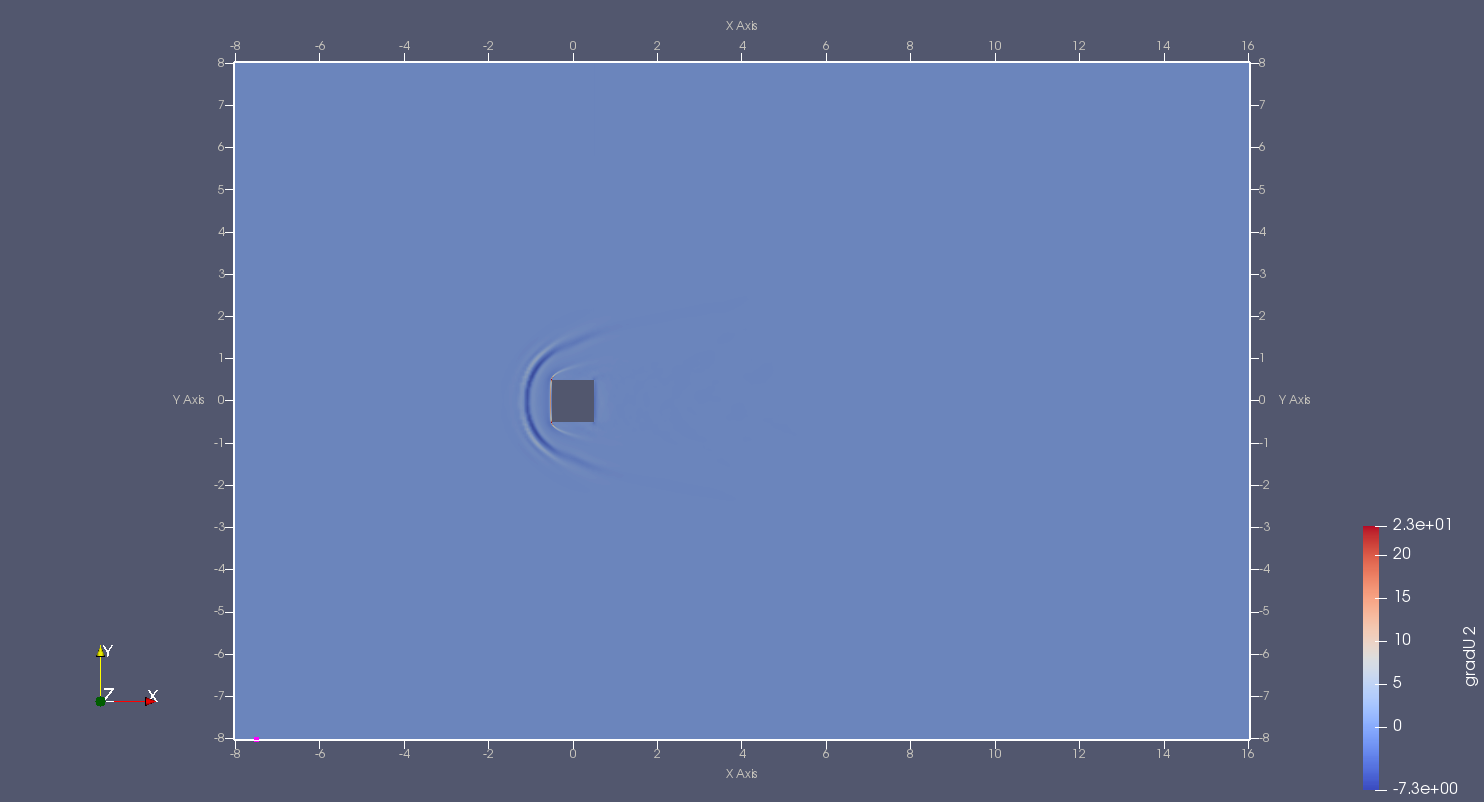
\includegraphics[width=0.45\textwidth]{figs/sqcyl/gradU/gradU2.png}}}%
    \qquad
    \subfloat[\centering R]{{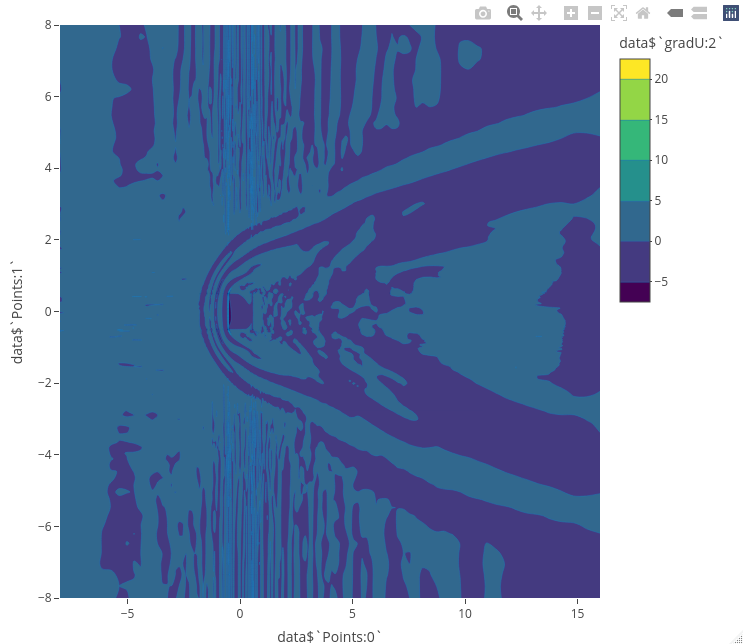
\includegraphics[width=0.3\textwidth]{figs/sqcyl/gradU_R/gradU2.png}}}%
    \caption{gradU2}%
    \subfloat[\centering OF]{{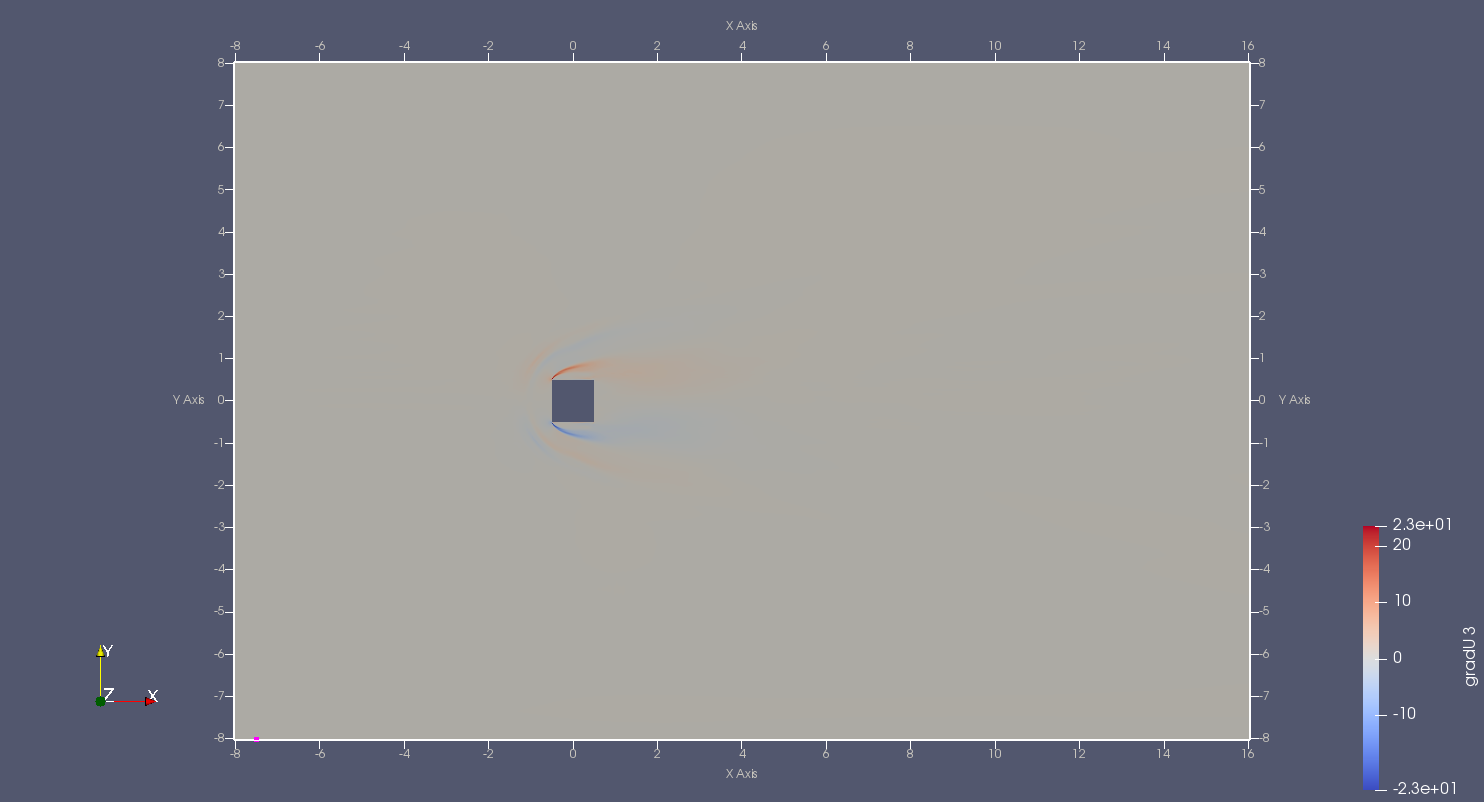
\includegraphics[width=0.45\textwidth]{figs/sqcyl/gradU/gradU3.png}}}%
    \qquad
    \subfloat[\centering R]{{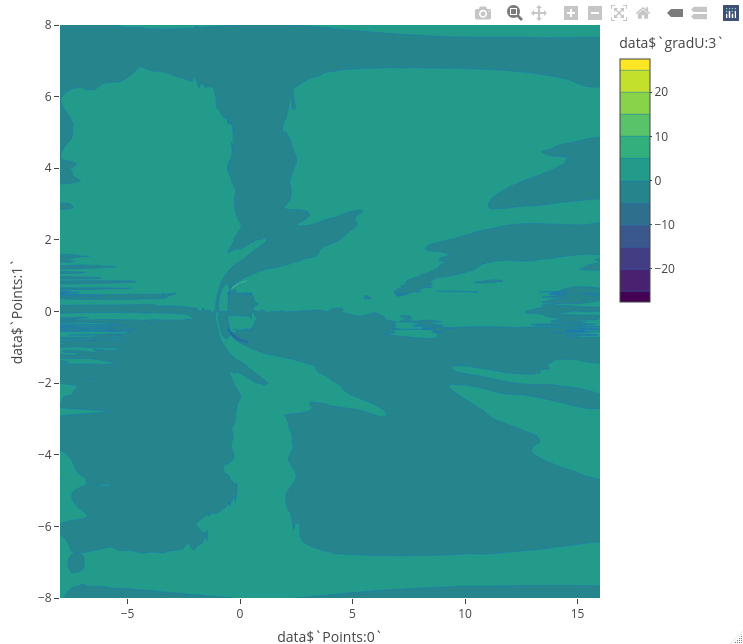
\includegraphics[width=0.3\textwidth]{figs/sqcyl/gradU_R/gradU3.png}}}%
    \caption{gradU3}%
    \subfloat[\centering OF]{{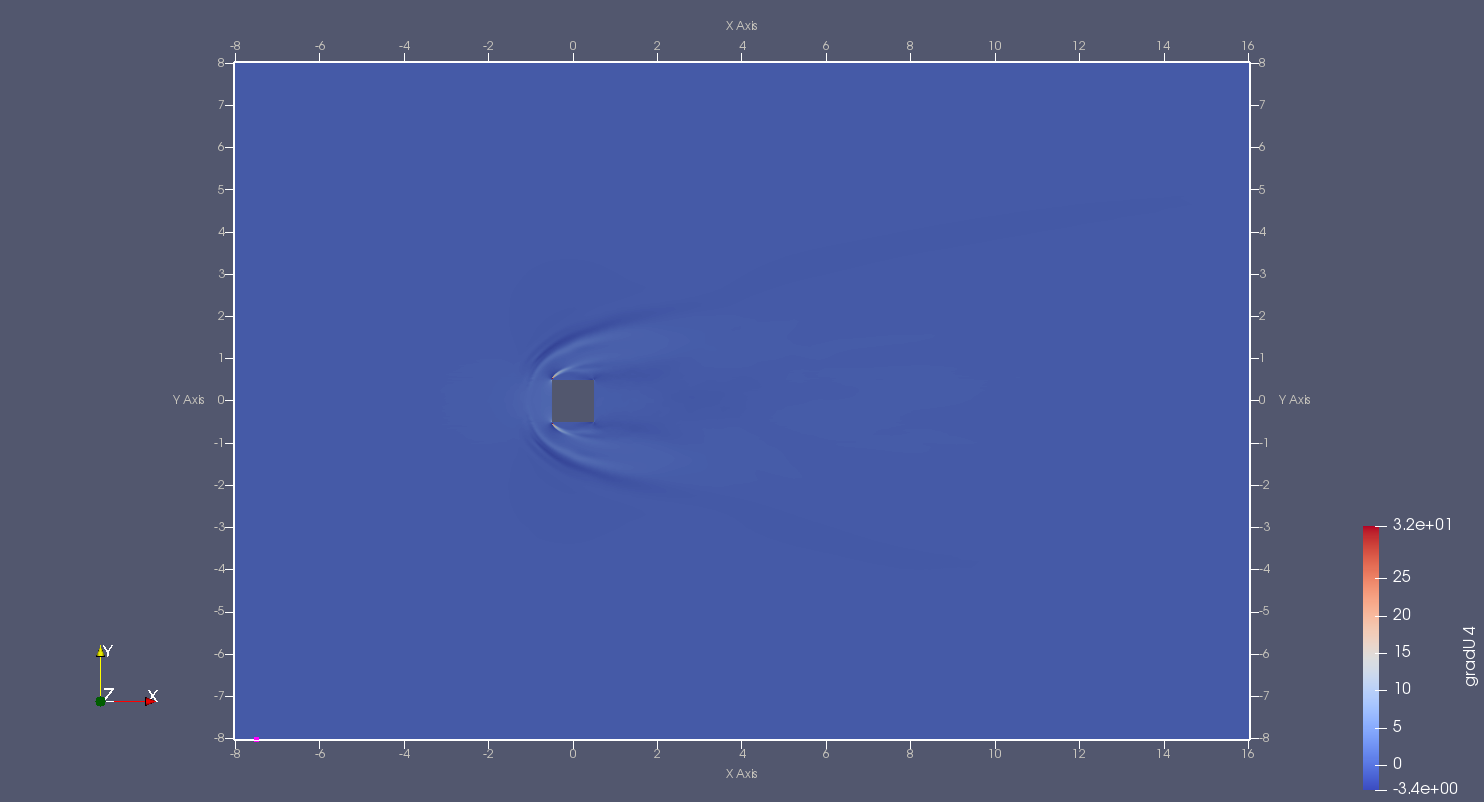
\includegraphics[width=0.45\textwidth]{figs/sqcyl/gradU/gradU4.png}}}%
    \qquad
    \subfloat[\centering R]{{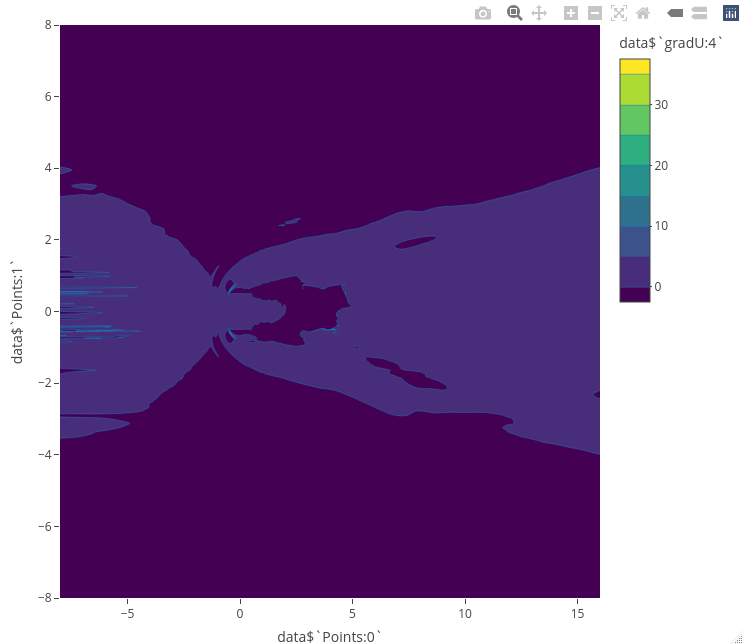
\includegraphics[width=0.3\textwidth]{figs/sqcyl/gradU_R/gradU4.png}}}%
    \caption{gradU4}%
    \label{fig:sqcyl:gradu}%
\end{figure}

\begin{figure}[H]%
    \centering
    \subfloat[\centering OF]{{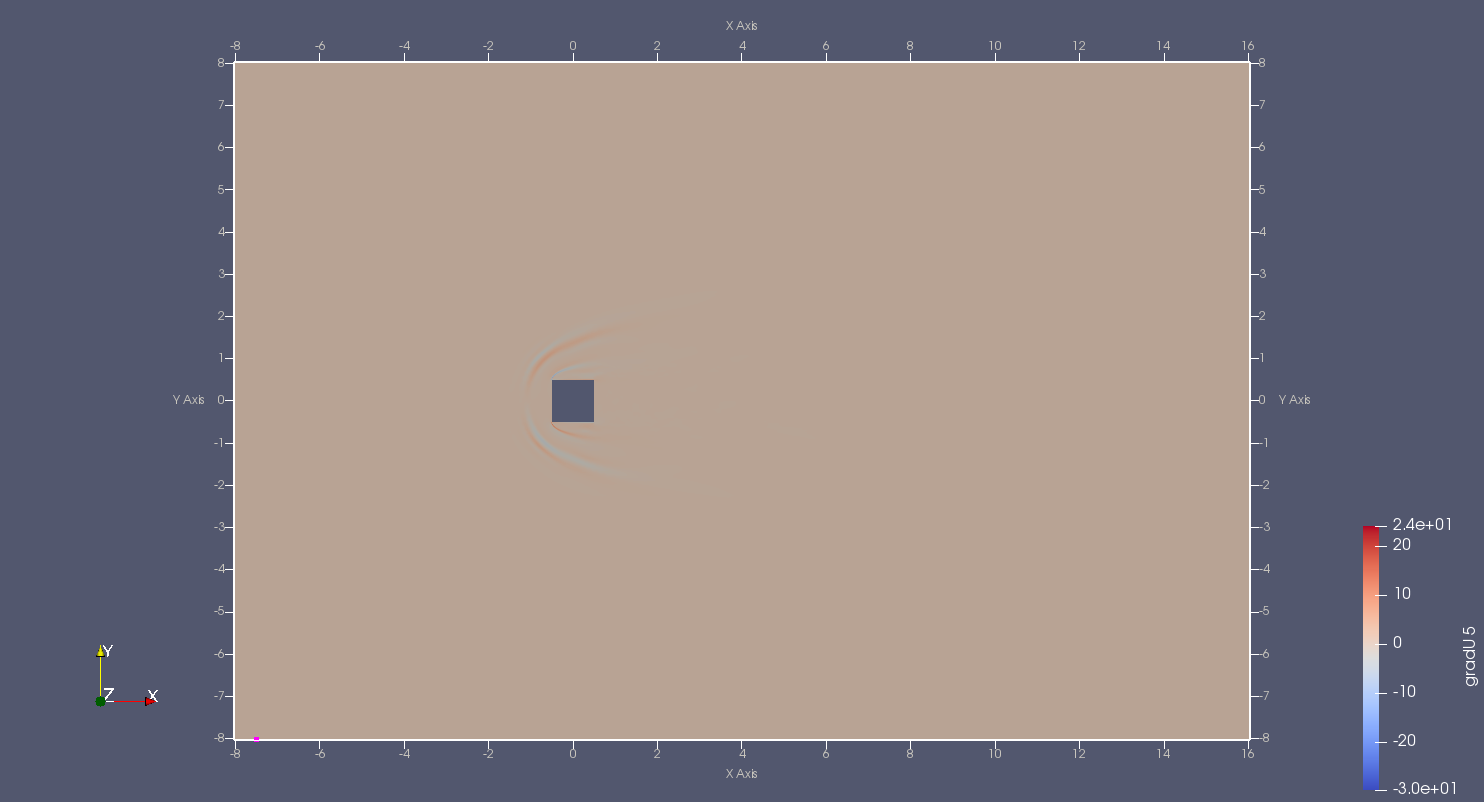
\includegraphics[width=0.45\textwidth]{figs/sqcyl/gradU/gradU5.png}}}%
    \qquad
    \subfloat[\centering R]{{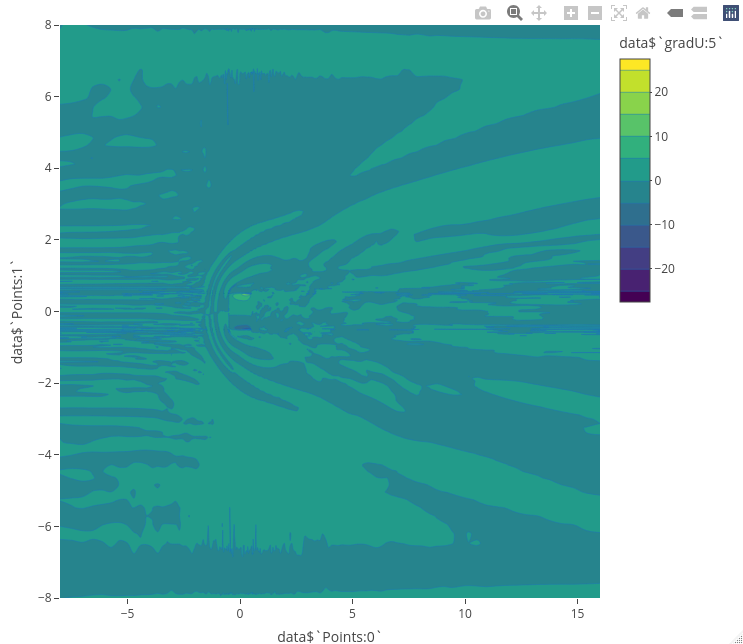
\includegraphics[width=0.3\textwidth]{figs/sqcyl/gradU_R/gradU5.png}}}%
    \caption{gradU5}%
    \subfloat[\centering OF]{{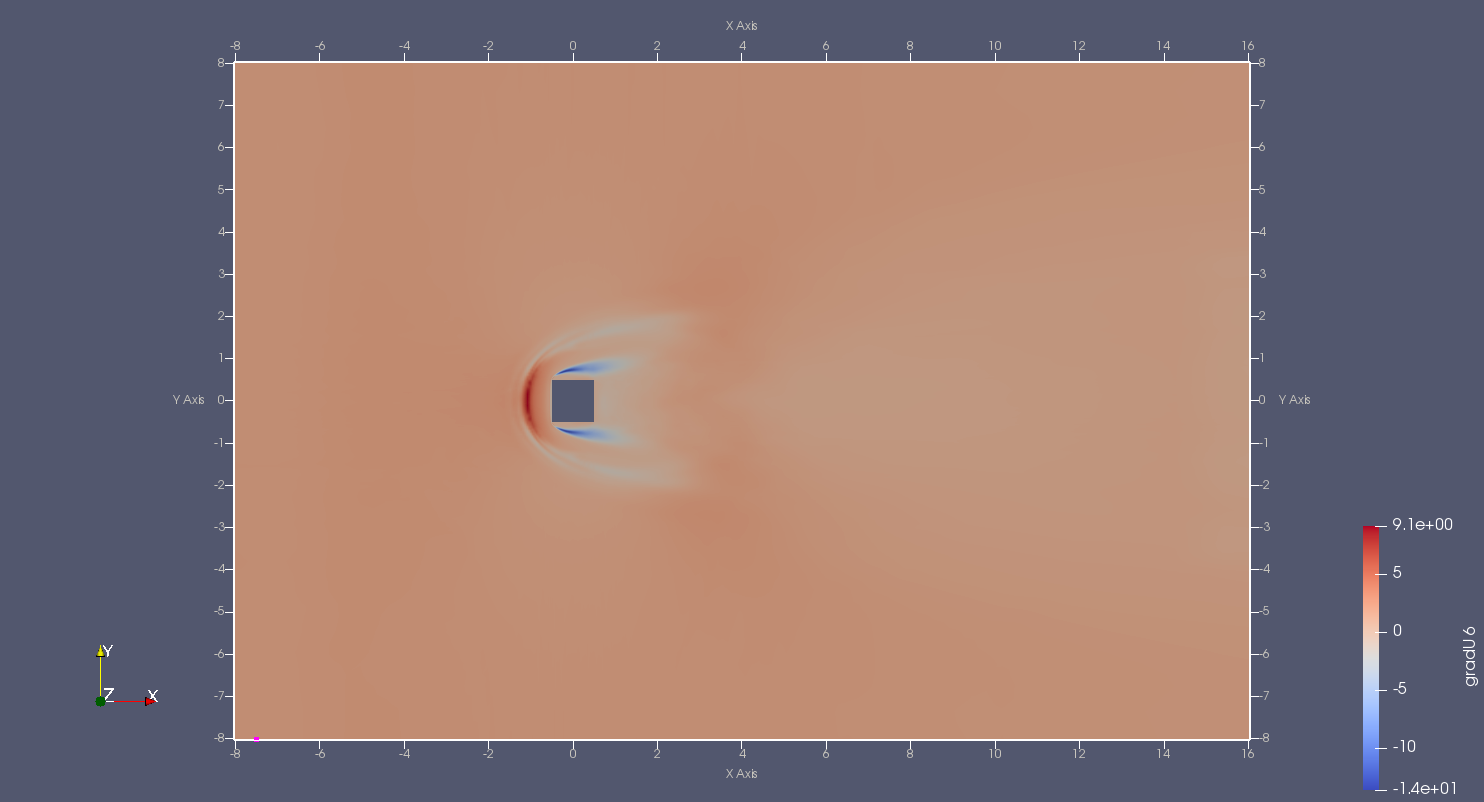
\includegraphics[width=0.45\textwidth]{figs/sqcyl/gradU/gradU6.png}}}%
    \qquad
    \subfloat[\centering R]{{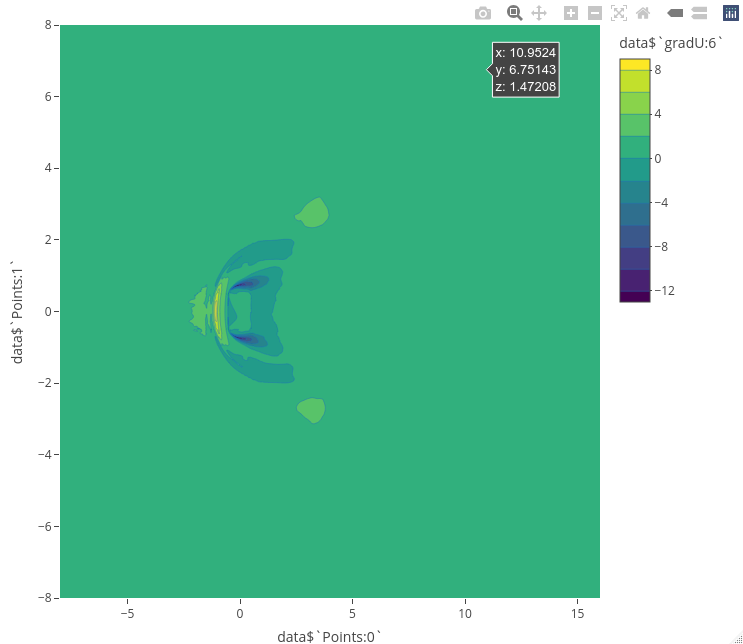
\includegraphics[width=0.3\textwidth]{figs/sqcyl/gradU_R/gradU6.png}}}%
    \caption{gradU6}%
    \subfloat[\centering OF]{{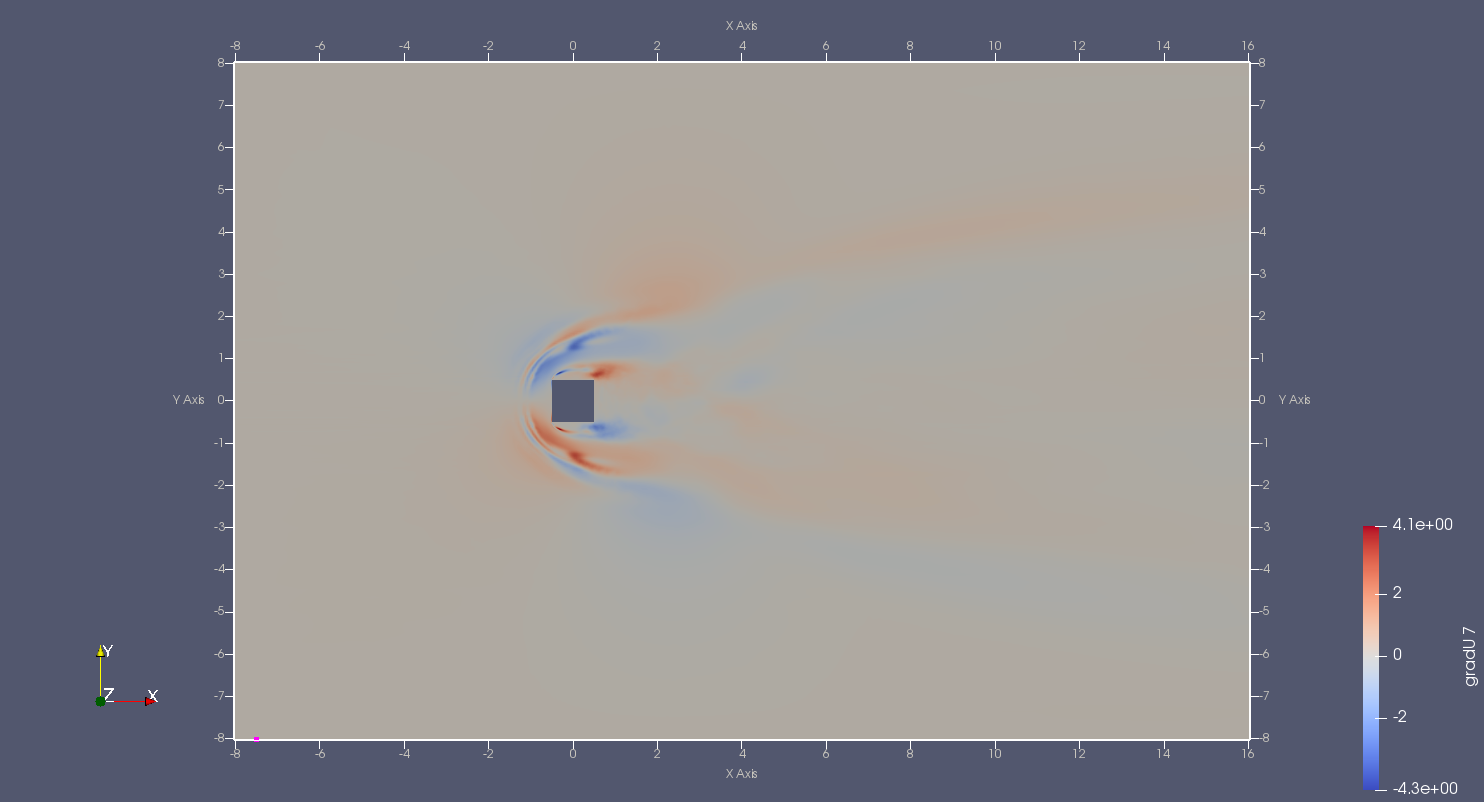
\includegraphics[width=0.45\textwidth]{figs/sqcyl/gradU/gradU7.png}}}%
    \qquad
    \subfloat[\centering R]{{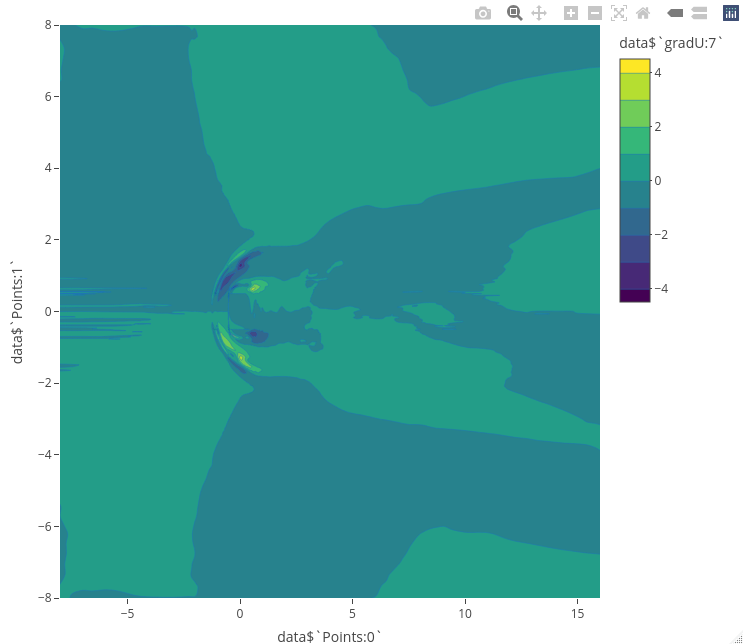
\includegraphics[width=0.3\textwidth]{figs/sqcyl/gradU_R/gradU7.png}}}%
    \caption{gradU7}%
    \subfloat[\centering OF]{{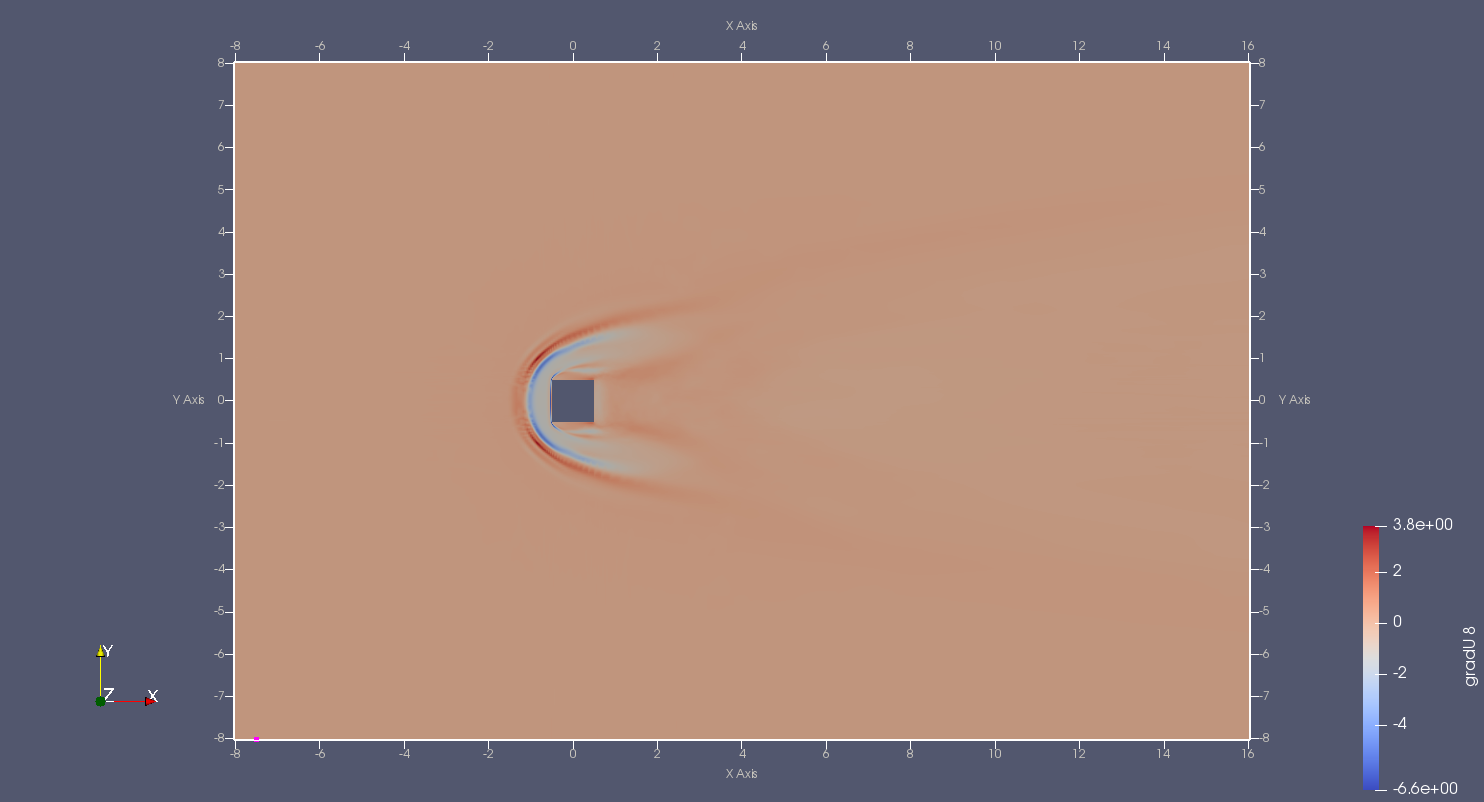
\includegraphics[width=0.45\textwidth]{figs/sqcyl/gradU/gradU8.png}}}%
    \qquad
    \subfloat[\centering R]{{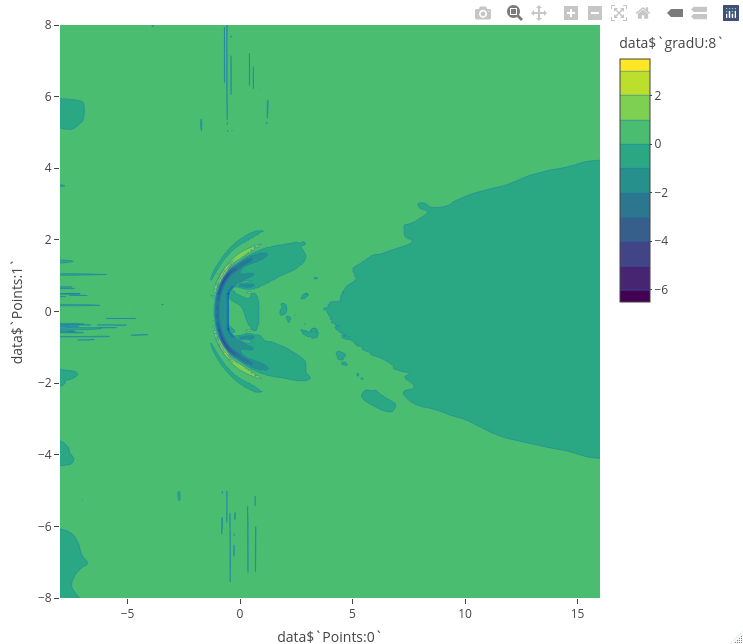
\includegraphics[width=0.3\textwidth]{figs/sqcyl/gradU_R/gradU8.png}}}%
    \caption{gradU8}%
    \label{fig:sqcyl:gradu}%
\end{figure}

\begin{figure}[H]%
    \centering
    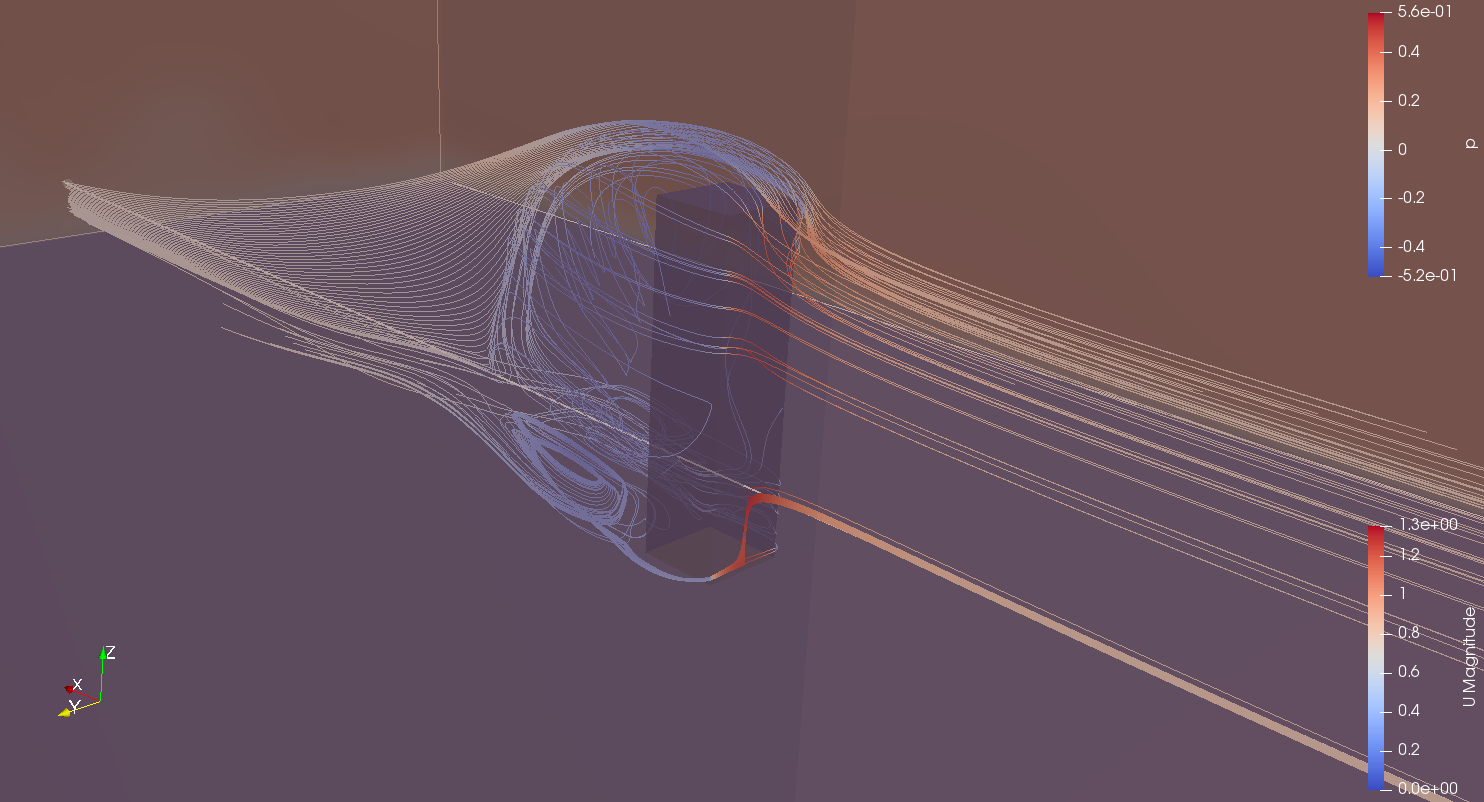
\includegraphics[width=0.9\textwidth]{figs/streamlines.png}
    \caption{Streamlines around a  a wall-mounted square cylinder. The velocity field is shown and the streamlines are coloured as the pressure field.}
    \label{fig:streamlines}%
\end{figure}

\begin{figure}[H]%
    \centering
    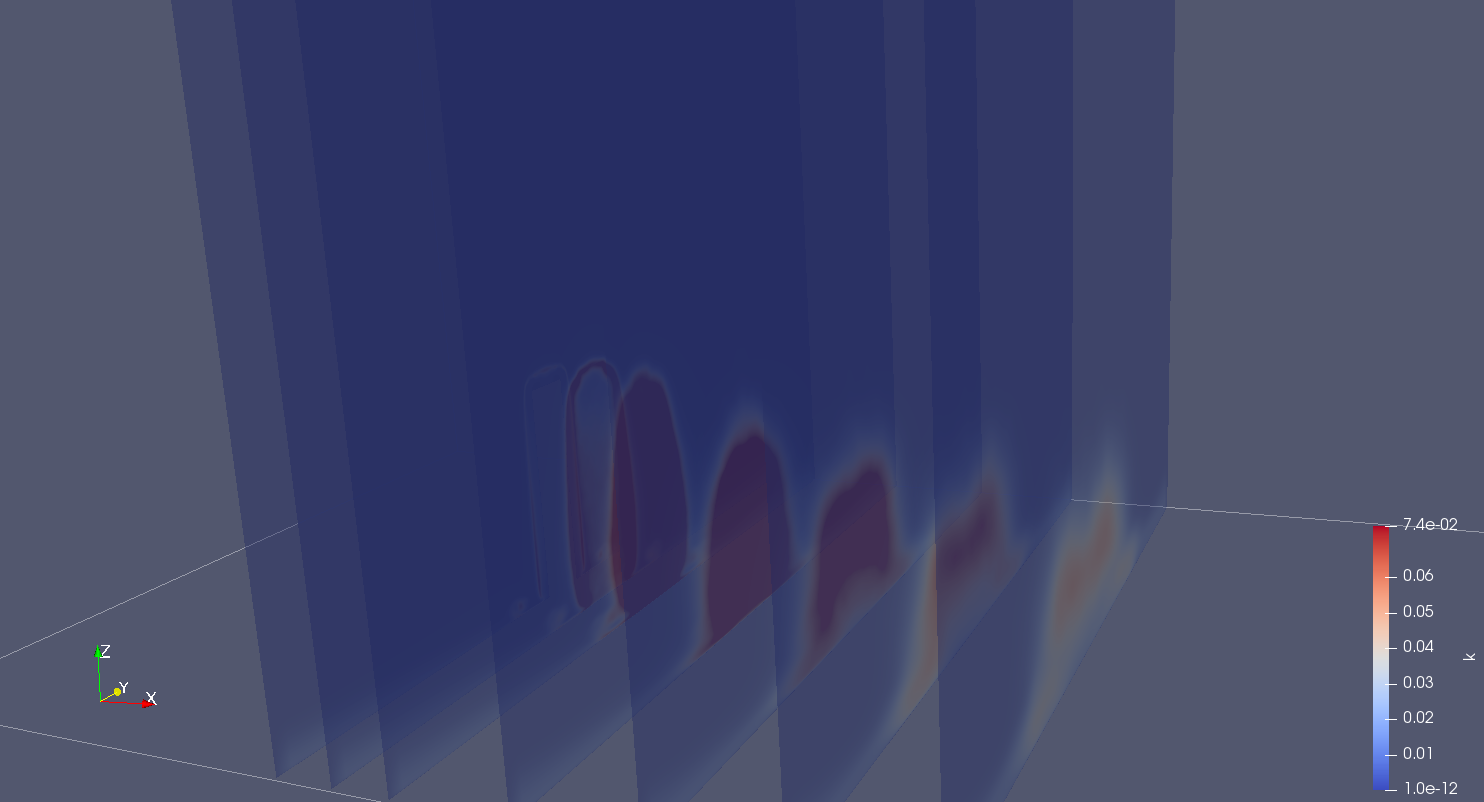
\includegraphics[width=0.9\textwidth]{figs/sqcyl/gradU/k_clips.png}
    \caption{Clips of the turbulence kinetic energy field $k$ for the wall-mounted square cylinder. Extractions planes at x = 0, 1, 2, 4, 6, 8, 10 m.}
    \label{fig:k_clips}%
\end{figure}

%\begin{figure}[H]%
%    \centering
%    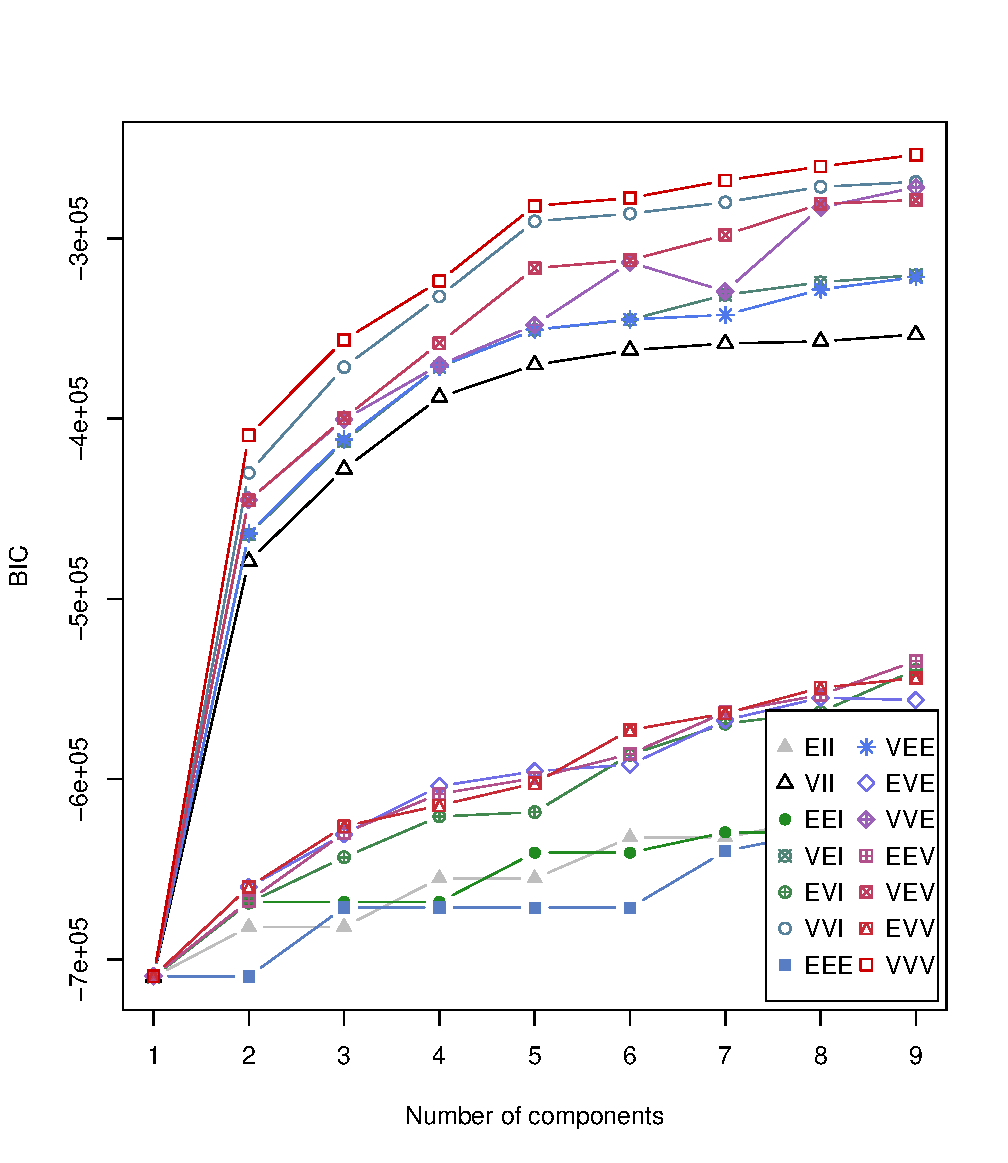
\includegraphics[width=0.9\textwidth]{figs/sqcyl/gradU_R/cluster/BIC.pdf}
%    \caption{BIC.}
%    \label{fig:bic}%
%\end{figure}
%\begin{figure}[H]%
%    \centering
%    \includegraphics[width=0.9\textwidth]{figs/sqcyl/gradU_R/cluster/classification.pdf}
%    \caption{Classification}
%    \label{fig:classification}%
%\end{figure}
%\begin{figure}[H]%
%    \centering
%    \includegraphics[width=0.9\textwidth]{figs/sqcyl/gradU_R/cluster/clusters_gradU6_7_8.pdf}
%    \caption{clusters}
%    \label{fig:clusters}%
%\end{figure}
%\begin{figure}[H]%
%    \centering
%    \includegraphics[width=0.9\textwidth]{figs/sqcyl/gradU_R/cluster/num_clusters.pdf}
%    \caption{Number of clusters}
%    \label{fig:numclusters}%
%\end{figure}
